\documentclass[12pt,a4paper,oneside]{book}
\usepackage[a-1b]{pdfx}
\usepackage{changepage}

\usepackage[utf8]{inputenc}
\usepackage[onehalfspacing]{setspace}

\usepackage{csquotes}
\MakeOuterQuote{"}

\usepackage{bm}
\usepackage{mathrsfs}
\usepackage{amsfonts}
\usepackage{amsmath}
\usepackage{amssymb}
\usepackage{gensymb}

\usepackage{algorithm}
\usepackage[noend]{algpseudocode}

\usepackage{float}
\usepackage{graphicx}
\usepackage[font={small,it}]{caption}

\usepackage{listings}
\usepackage{color}

\usepackage[sectionbib]{natbib}
\usepackage{chapterbib}

\usepackage{emptypage}
\usepackage{fancyhdr}
\pagestyle{fancy}
\fancyhead[L]{}
\fancyhead[R]{\leftmark}

\setlength{\headheight}{15pt}

\definecolor{mygreen}{rgb}{0,0.6,0}
\definecolor{mygray}{rgb}{0.5,0.5,0.5}
\definecolor{mymauve}{rgb}{0.58,0,0.82}

\lstset{
  basicstyle=\ttfamily\footnotesize,
  backgroundcolor=\color{white},   % choose the background color; you must add \usepackage{color} or \usepackage{xcolor}
  breakatwhitespace=true,         % sets if automatic breaks should only happen at whitespace
  breaklines=true,                 % sets automatic line breaking
  %captionpos=b,                    % sets the caption-position to bottom
  commentstyle=\color{mygreen},    % comment style
  deletekeywords={...},            % if you want to delete keywords from the given language
  escapeinside={\%*}{*)},          % if you want to add LaTeX within your code
  extendedchars=true,              % lets you use non-ASCII characters; for 8-bits encodings only, does not work with UTF-8
  frame=L,                    % adds a frame around the code
  keepspaces=true,                 % keeps spaces in text, useful for keeping indentation of code (possibly needs columns=flexible)
  keywordstyle=\color{blue},       % keyword style
  language=Python,                 % the language of the code
  morekeywords={*,...},            % if you want to add more keywords to the set
  numbers=left,                    % where to put the line-numbers; possible values are (none, left, right)
  numbersep=15pt,                   % how far the line-numbers are from the code
  numberstyle=\tiny\color{mygray}, % the style that is used for the line-numbers
  rulecolor=\color{black},         % if not set, the frame-color may be changed on line-breaks within not-black text (e.g. comments (green here))
  showspaces=false,                % show spaces everywhere adding particular underscores; it overrides 'showstringspaces'
  showstringspaces=false,          % underline spaces within strings only
  showtabs=false,                  % show tabs within strings adding particular underscores
  stepnumber=1,                    % the step between two line-numbers. If it's 1, each line will be numbered
  stringstyle=\color{mymauve},     % string literal style
  tabsize=2,                       % sets default tabsize to 2 spaces
  %title=\lstname                   % show the filename of files included with \lstinputlisting; also try caption instead of title
  belowskip=50pt
}

%\graphicspath{ {img/} }

\begin{document}

\evensidemargin 1.4cm
\oddsidemargin 1.4cm

	\begin{titlepage}
\begin{adjustwidth}{-1cm}{-1cm}

\begin{figure}
\begin{center}

\includegraphics[width=4cm,height=4cm]{img/0_logo_units.png}
\vspace{0.2cm}
\end{center}
\end{figure}

\begin{center}
\textsc{\LARGE University of Trieste } \\
\vspace{0.1cm}

{\large Department of Mathematics and Geoscience}\\
\vspace{1cm}

\textsc{\Large Master Degree in \\Data Science and Scientific Computing}\\

\vspace{2cm}

\begin{large}
\begin{center}
\textbf{\Large Adversarial Learning of Robust and Safe Controllers for Cyber-Physical Systems}
\end{center}
\end{large}

\vspace{2cm}

\begin{normalsize}
\begin{tabular}{l c r}
{\it Author: } & &{\it Supervisor:} \\
\vspace{0.5cm}
{\it Francesco Franchina} & \hspace{5cm} &{\it Luca Bortolussi} \\
& \hspace{3cm} & {\it Cosupervisors:} \\
& \hspace{3cm} & {\it Francesca Cairoli} \\
& \hspace{3cm} & {\it Ginevra Carbone} \\

\end{tabular}
\end{normalsize}

\vspace{1.5cm}

\line(1, 0){370} \\
\begin{normalsize}
\textsc{Academic Year 2018/2019 - April 2020}
\end{normalsize}

\end{center}

\end{adjustwidth}
\end{titlepage}


	\hbox{}
\thispagestyle{empty}
\newpage 

	\thispagestyle{empty}
	\null \vspace{\stretch{1}}
	\begin{flushright}
	\emph{ Alle persone che tengo sempre vicino al cuore \\ che, anche nelle tempeste, riescono a donarmi tranquillità. \\ A tutti coloro che hanno caratterizzato questa mia esperienza triestina. \\ Grazie! }
	\end{flushright}
	\vspace{\stretch{2}}\null 

\hbox{}
\thispagestyle{empty}
\newpage 

	\tableofcontents

\setstretch{1.4}

    \chapter*{Abstract}
\addcontentsline{toc}{chapter}{Abstract}

Data-driven models are bringing huge advantages in terms of performance and effectiveness in many sectors.
In the field of Cyber-Physical Systems, although, they are not widespread since their opaqueness and lacks formal proofs pose a serious threat to their employment.

We propose and analyze a novel approach in creating robust and safe controllers drawing from the literature of the adversarial learning.

Our method trains in an adversarial way two Neural Networks to reach a twofold goal:
obtain one network that is able to generate difficult configurations of the environment and another that is able to overcome them in a safe e robust way.
The aim is to create a formally verified controller and, at the same time, to give insights on the most demanding corner cases of a given model.

The approach is promising and worthy of further investigation.


\chapter*{Abstract in italiano}
\addcontentsline{toc}{chapter}{Abstract in italiano}

I modelli data-driven stanno permettendo di raggiungere efficacia e performance mai viste prima in molti settori.
Tuttavia, nel campo dei Cyber-Physical System non sono ancora molto impiegati dal momento che, per via del loro funzionamento difficilmente formalizzabile, non permettono di fare le adeguate verifiche di sicurezza che li renderebbero delle valide alternative ai sistemi attualmente in uso.

Noi proponiamo e analizziamo un nuovo approccio alla creazione di controllori robusti e sicuri attingendo dalla letteratura dell'apprendimento avversario.

Il nostro sistema addestra due Reti Neurali avversarie per ottenere un duplice obbiettivo: ottenere una rete in grado di generare configurazioni insidiose dell'ambiente e un'altra rete in grado di affrontare tali situazioni in modo robusto e sicuro.
Lo scopo è quello di ottenere un controllore verficato formalmente e, allo stesso tempo, ottenere informazioni su quali sono i casi più difficili da gestire per un dato modello.

Il nostro approccio è promettente e sicuramente degno di ulteriori approfondimenti.

	\chapter{Introduction}

This work is highly interdisciplinary and aims at using advanced frameworks like Generative Adversarial Networks and formal methods for model verification to propose a new approach on how to learn safe and robust controllers for Cyber-Physical Systems.

The challenges for creating truly autonomous and safe system are currently being actively investigated and we believe that our method could give some concrete contribution to the already flourishing literature on this topic.


\section{Context}
Every day we unconsciously use of an increasing number of automatic systems that have not been programmed explicitly.
They have been virtually trained on human examples in order to learn the proper behaviour in the most common scenarios.
The massive usage of Deep Neural Networks to solve many of today's challenges \cite{Dargan_Kumar_Ayyagari_Kumar_2019} is a striking example of how effective this approach can be.
The adoption of such technologies is growing in both industrial and consumer sectors and we are increasingly relying on data-driven models that work very well but that, due to their complexity, we fail to understand in their whole \cite{Carvalho_Pereira_Cardoso_2019}.

This practice brought numerous advantages like speed and precision in the most common cases but, once we test the models in some unusual environment or with some weird configurations, they can fail miserably.
While in some field of application this can be quantified as an economic loss, in others the situation is much more delicate, especially in those where human health is involved.

Due to such practical reasons, the development of advanced models is confined to controlled environments and, usually, it is not a viable option in those that would benefit from automation, like the big complex artificial systems on which we daily rely on: transportation, power grid, production and so on.

The biggest challenge for the deployment of autonomous systems that can have a larger impact in everyday life, is posed by the complexity of the exploration of \textbf{open worlds} like ours.
\textit{Open worlds}, in fact, are difficult to model and control due to the significant amount of stochastic variables that are needed in their modelling and the variety of unpredictable scenarios that they present.
Therefore, while trying to ensure safety and robustness, we need to be cautious about not trading them with the models' effectiveness.


\section{Problem statement}
When it comes to the control of Cyber-Physical Systems, the industry tends to rely on well-established and well-understood techniques, belonging to classic Control Theory \cite{pidrulez}.
These algorithms allow a high degree of predictability along with good robustness in presence of noise.

Nevertheless, research is trying to fill the gap with Deep Learning \cite{deepqlearning} that, on one hand, guarantees more flexibility and resilience but on the other sacrifices the full comprehension of the whole model.
The big problem posed by a partial comprehension of the model is the impossibility of checking the behaviour of the controller in the case of unpredictable scenarios that could lead to unintended or harmful behaviours.

Finding an efficient, safe and comprehensible solution is still an open challenge that offers a large space for improvements and fertile ground for new ideas.

\section{Contributions}
Most of the research that combines the usage of Deep Learning for robust control is done in the field of Reinforcement Learning \cite{brief_rl}.
It offers different approaches, but the most promising trend involves learning from an \textit{expert} how to face the most common scenarios \cite{inverserl}.
This approach performs reasonably well but presents some limits in case of unexpected situations.

What we are going to investigate is the possibility of autonomously learning a safe and robust controller in a \textit{open world scenario}.
The proposed approach consists in the training of two Neural Networks and is inspired by Generative Adversarial Networks \cite{gan_2014}. The two networks have opposite roles: while the \textit{attacker} tries to generate troubling scenarios for the controller, the \textit{defender} learns how to face them without violating some safety constraints.

The outcome of such training procedure is twofold: on one side we get a robust controller, on the other we get a generator of adverse tests.


\section{Structure}
After covering the background knowledge required to understand the whole architecture, we will show the proposed solution.
Later, we will show the case studies on which we tested our model and the respective results.
Finally, we will draw some conclusions about this work and its possible future development.
	
	% chapters
	\chapter{Background}

This project is quite broad and combines knowledge coming from different fields.
Here we cover the theoretical background required to understand it.

\section{Cyber-Physical Systems}

The field of CPS, Cyber-Physical Systems, is relatively new: the name was coined and started gaining ground only in the first decade of the 2000s.
The knowledge employed in this field, however, comes from well-known disciplines: CPS is, in fact, a highly interdisciplinary area where Physics, Control Theory, Embedded Systems, Formal Verification and Robotics.

Despite the recent foundation of this field, the first medical devices that can be classified as CPS are quite dated: pace-makers and insulin-pumps, for instance, were invented around the '60s.
Due to the increasing computational power of the controllers classified as Edge Computing \cite{edge_comp_2016} and to the new possibilities given by the advent of the Internet of Things, we are going to hear about CPS new fields of application: they are already effectively used in growing fields like automotive, manufacturing, energy management and in any other field that involves the employment of robots \cite{Sanislav_Miclea_2012}.

Each of this fields deals with \textit{Complex Systems} in which \textbf{continuous}, \textbf{discrete} and \textbf{stochastic} processes are involved.

\subsection{Definition}
As the name suggests, a Cyber-Physical System is composed of two parts:
\begin{itemize}
  \item the "\textbf{cyber}" one is a computational system that processes logical operations,
  \item the "\textbf{physical}" one is the real phenomenon that we are modelling.
\end{itemize}
We define it CPS only when the two components are deeply interconnected by some communication devices that can affect each other's state.

The major difference between the two components is their way of dealing with time.
The \textit{cyber} part operates in a discrete time-scale where the internal state of the model is governed by the execution of algorithms.
The \textit{physical} part, instead, lives in a continuous time-scale where the model's state evolves according to the physical laws of nature.

The communication between the two components of the CPS takes place through \textbf{transducers}, allowing the exchange of information between them.
This allows the two parts to co-evolve simultaneously following their respective rules: the instructions of the algorithm for the \textit{cyber} part and physical laws the \textit{physical} one.

\textbf{Sensors} are transducers that discretize an analog signal, therefore, they allow the flow of information from the \textit{physical} part to the \textit{cyber} part.
For instance, we call \textit{sensor} whatever is able to digitally measure a property of the physical world: thermometers, photoresistors, camera sensors, etc.

\textbf{Actuators}, instead, are transducers that use a digital input to transform the physical world.
They work in the exact opposite way with respect to \textit{sensors}, in fact, they allow the information from the \textit{cyber} part to flow toward the \textit{physical} one.
Examples of actuators are all those devices that, given a digital input, can produce an observable change in the world: motors, speakers, electromagnets, etc.

\begin{figure}[H]
	\centering
	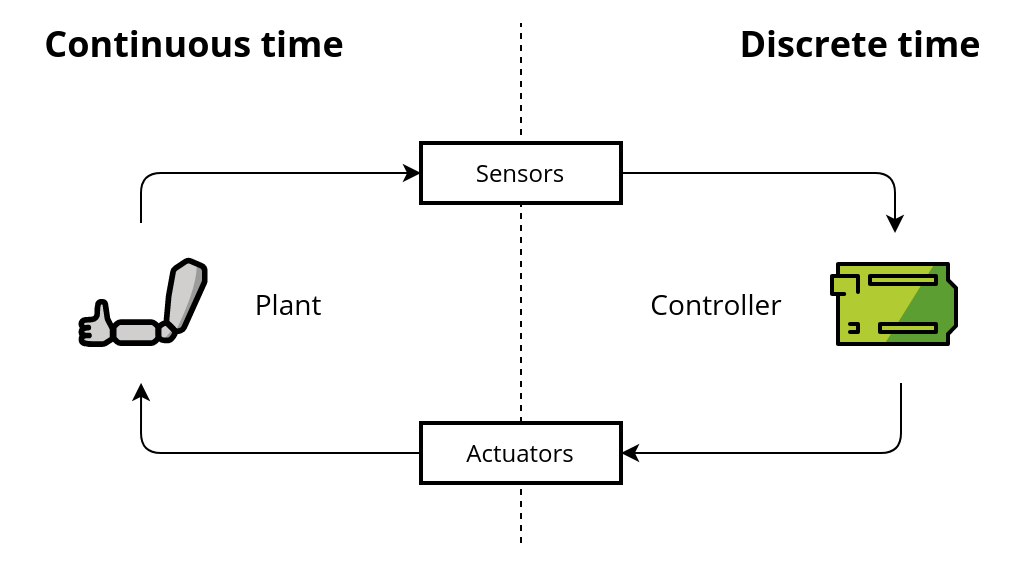
\includegraphics[width=11cm, keepaspectratio]{img/2_1_cps.png}
	\caption{The two components of a CPS interact through sensors and actuators, these allow them to exchange information and act as a single system.}
\end{figure}

The communication between the two parts is fundamental because a CPS acts as a whole due to the constant flow of information that allows the two parts to adapt to each other.
We are now going to describe a practical example of CPS: the \textit{cruise-control}, whose aim is to keep constant the speed of a vehicle.

\subsection{Physical component}
In the cruise-control example, the vehicle and its dynamic represent the physical part of the CPS.
This part is often referred to as the \textbf{plant}.
We call \textit{state} a specific configuration of the variables describing the model's properties we are interested in.
For instance, in the cruise-control problem, the \textit{state} is composed of the vehicle's speed $v$ and the \textit{steepness} of the road $\theta$.
The \textit{plant} evolves its \textit{state} in time according to the physical laws involved.

\begin{figure}[H]
	\centering
	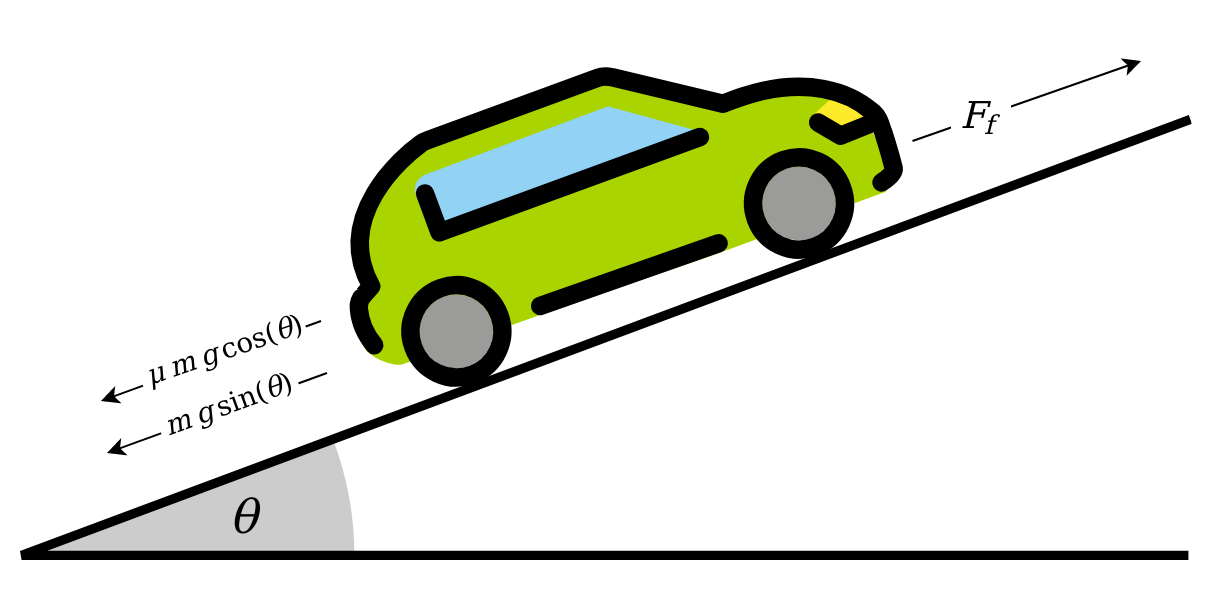
\includegraphics[width=11cm, keepaspectratio]{img/2_1_car_physics.png}
	\caption{The physical forces involved in the cruise-control problem.}
\end{figure}

In this case we can describe the evolution of the vehicle's \textit{state} through a differential equation that captures the continuous time-scale of the behaviour:
$$ m\frac{dv}{dt} = \frac{F_f}{m} - mg \sin(\theta) - \mu mg \cos(\theta) $$

In the equation above, $F_f$ is variable that we can control: it is the force that pushes the vehicle forward, directly proportional to the amount of fuel provided to the engine.
Apart from the inclination of the road $\theta$, all the other symbols that appear in the equation are constants: the vehicle's mass $m$, the gravity $g$ and the friction constant $\mu$.
The equation shows the link between the variable that we can control and the rest, the \textit{environment}.
By knowing the properties of the \textit{environment}, therefore, it is possible to compute deterministically the value of the input $F_f$ for which the speed of the vehicle $v$ remains constant.

The physical model of a system should be able to describe the relationship between all the variables that are involved in its dynamics.
The more complex a system is, the more complex are its equations.

\subsection{Cyber component}
The \textit{cyber} part of the CPS is referred to as the \textbf{controller}.
Its role is to plan how the system should behave in order to achieve its goal by executing a pre-programmed algorithm.
In our example of cruise-control, the aim of the \textit{controller} is to keep the velocity constant.

The \textit{controller} is -- usually, but not always \cite{JIISc-9303_distrCPS} -- an embedded computer that executes a sequence of programmed operations in a discrete time-scale.
The way of modelling the algorithmic part draws directly from the literature of embedded systems \cite{design_embedded_sys}, where the employed formalisms -- like \textit{Finite State Machines} (FSM) or other kind of more complex finite-state automata -- have been refined over the years.

This kind of formalism describes how the \textit{cyber} part evolves in time through the discrete \textit{states}.
The \textit{state} changes \textbf{deterministically} when a certain internal (a timer, for instance) or external (a value form a sensor) condition is met.
Moreover, it can change in a \textbf{stochastic} way if the transition happens randomly according to a specific probability distribution.

\textit{Sensors} and \textit{actuators} play a crucial role for the \textit{cyber} part since, through them, it can get information about the \textit{physical} part's state and compute how to control the actuators to reach -- or get closer to -- the desired state.
For instance, in the cruise-control problem, the \textit{controller} receives information about the current state of the physical system through the \textit{speedometer} and, according to its algorithm, manages how much fuel to provide to the engine to keep the speed constant.

\subsection{Hybrid model}
Due to the twofold nature of the CPSs, they can be represented as \textbf{Hybrid models}.
The name \textit{hybrid} comes from the fact that we include in the same model both continuous and discrete systems.
In the example of the cruise-control, in fact, we have the continuous state's variable of the velocity that determines whether the controller should or should not (Boolean variable), provide more fuel to the engine.

\textit{Hybrid models} can be formalized using \textbf{hybrid automata}.
In a \textbf{hybrid automaton}, like in the FSM, each \textit{state} can change deterministically or randomly.
Such formalism extends the FSMs by allowing conditions on the continuous variables observed from the CPS' physical part. 
In this way, it is possible to model even a fairly complex interaction scheme in a compact way.

\begin{figure}[H]
	\centering
	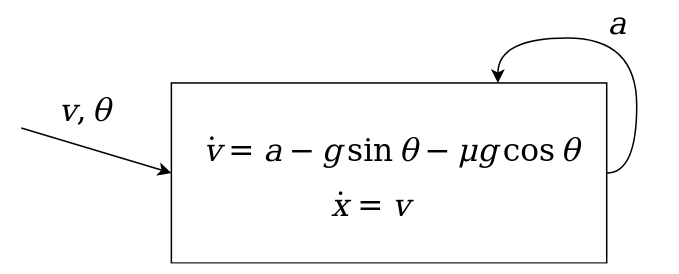
\includegraphics[width=8cm, keepaspectratio]{img/2_1_hybridmod.png}
	\caption{This hybrid model handles the problem of the cruise control. It has only one state and takes as input the vehicle's velocity $v$ and the road's steepness $\theta$. It gives as output the acceleration $a$ that updates the state of the system. The other terms that appear are constants: $\mu$ is the friction constant and $g$ is the gravity.}
\end{figure}


\subsection{Modelling and Design}
The modelling of the continuous part consists in obtaining the equations that appropriately describe the behaviour of the \textit{plant}.
With the aim of deriving the equations involved in the problem, we need to consider the relevant dynamics that take place into our setting.
Once we obtain the differential equations that describe the system, we can make some considerations on its controllability and, in particular, on the way the control should occur.

The modelling of the discrete part, instead, aims at identifying the possible discrete \textit{controller}'s states.
This procedure is fundamental to obtain the FSM that can completely represent the \textit{controller}.
The implementation of the FSM as an algorithm is often not-trivial due to the many machine's limitations: memory, compute power, precision and execution's speed are all finite resources.

In particular, the last constraint has become an important bottleneck that is preventing CPS from scaling massively \cite{realtimecps}.
When designing a controller, in fact, it's very important to take into account the latency that will occur between the moment in which the sensors will get information about the state and the moment in which the actuators can react accordingly, after that the \textit{controller} has determined the strategy to follow.
In \textit{time-critical} systems this latency should be kept as low as possible in order to keep the system into a safe state and deliver the response action in time.
Traditional methods are still able to stand out with respect to the newer counterparts due to the fact that the most sophisticated control techniques require complex algorithms that, sometimes, cannot run fast enough to make the system a \textit{real-time} one \cite{pidrulez}.

A fundamental part of the design process consists in paying attention to the kind of feedback we expect to receive from the system once that the planned action has taken place through the actuators.
There are two possible choices: designing an \textit{open-loop system} or a \textit{closed-loop system}.

In an \textbf{open-loop} system there is lack of feedback: there is no way for the controller to check whether a given action actually took place or not.
Of course the limits of this approach are evident but they can work reasonably good in certain scenarios.
Examples of \textbf{open-loop} systems are many appliances that, once that they have been instructed on what to do, they execute the program and terminate.
On the other hand, the advantages are lower complexity and fewer resources needed.

A \textbf{closed-loop} system, instead, is characterized by the feedback's presence right \textbf{after} the action has occurred.
The purpose of the feedback is to check whether the action actually brought the system into the desired state or if it still needs more operations in order to reach it.
These kind of systems are \textit{adaptive} and more reliable respect to the \textit{open-loop} ones since they can detect unexpected behaviours and handle them adequately.
By contrast, these kind of systems are more expensive since they require specific sensors and control algorithms in order to provide the feedback.

\begin{figure}[H]
	\centering
	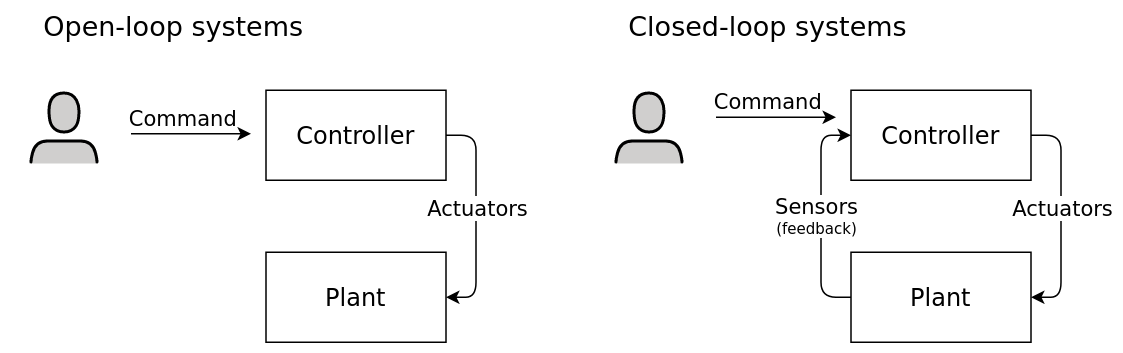
\includegraphics[width=12cm, keepaspectratio]{img/2_1_openclosed_loop.png}
	\caption{Illustration of the difference between open-loop systems and closed-loop systems. The term closed-loop refers precisely to the circular communication that is present in the system.}
\end{figure}

Once we have modelled the whole CPS, it is possible to build software simulators of both the continuous and discrete dynamics in order to test the performance and the capabilities of the system.

\subsection{Safety and monitoring}

The interest in CPS is steadily growing, and as such the research landscape of CPS is complex and rich \cite{Greer2019CyberPhysicalSA}.
One theme receiving a lot of attention is that of CPS \textit{safety} and \textit{security}.
While \textbf{security} is about preventing malicious attacks of the CPS \cite{cps_sec}, \textbf{safety}, in particular, concerns the behaviour of CPS and their interaction in an open world, which should be safe and not lead the CPS device or other interacting agents -- especially humans -- to accidents. 
Safety can be framed in a formal setting by requiring a CPS to satisfy a given set of formal requirements, describing in a mathematically sound way properties like "the autonomous vehicle never bumps into a human" or "the vehicles's speed should always remain close to $50km/h$", in the case of the cruise-control.

A popular language to specify safety properties is Signal Temporal Logic \cite{stl2004}, a \textit{temporal logic} tailored to deal with continuous quantities that we are going to cover more in detail in the last section of this chapter. 
Given a STL property, in principle, we would like to formally verify that it holds for the CPS under consideration, or at least for its mathematical model.
This means having a formal proof that each trajectory of the model is safe.
Such procedure is named \textbf{verification} or \textbf{model checking}.
Verification of STL properties on hybrid systems, however, is often undecidable or just computationally too complex -- especially in the case of \textit{stochastic models} -- therefore it is an active field of research \cite{Zheng_Julien_2015}.

In such cases a common approach is that of \textbf{monitoring} the system trajectories at \textit{run-time} with STL properties and leveraging this information to assess safety in a weaker way, e.g. only with statistical guarantees. 

Another technique to assess the safety of a CPS is \textbf{falsification}.
This technique applies \textit{monitoring} to simulations specifically conceived in order to drive the system to an unsafe state \cite{cps_falsification}.
STL propositions are used to identify the dangerous corner-cases that can be used as \textit{counterexamples} for gaining insight on how the problem occurred and to tune the model's parameters accordingly \cite{counter-tuning} or to train the model to avoid such cases \cite{counter-train}.


\section{Generative Adversarial Networks}

A Generative Adversarial Network (GAN) is a \textbf{generative model}, a class of statistical models whose aim is to learn the probability distribution of the input data.

In particular, this family of models learns a mapping function between a given distribution $P_z$ and the distribution learnt from the data $P_{latent}$.
The learning procedure is supervised and aims at reducing the difference between the generative distribution $P_{latent}$ and the dataset distribution $P_{data}$.
A peculiar characteristic of these models is that, once the learning procedure has been completed, it is possible to sample from them using the noise distribution $P_z$.

Summarizing, a generic \textit{generative model} takes as input a noise vector $z \sim P_z$ and maps it to a sample drawn from the distribution $P_{latent}$, learnt from the data distribution $P_{data}$.
The term "generative" refers to the capability of the model of \textbf{generating} new artificial samples that resemble the provided ones.

GANs, in particular, use NNs and a specific learning approach in order to learn the mapping function between the two distributions.
In the following sections we are going to cover the concepts used by GANs.

\subsection{Neural Networks}
The concept behind Neural Networks (NNs) is quite old despite only in the last decade the related literature is flourishing \cite{nn_survey}.
This is happening because of the availability of \textit{big data} and the increased computational power allow a faster and more accurate training, allowing their employment to deal with increasingly complex problems.
The ancestors of the modern NNs root their history in the '50s, when scientists begun understanding and formalizing how biological neurons work \cite{Rosenblatt58theperceptron}.

\subsubsection{Perceptron}
The term \textit{perceptron} was coined during the '50s and its way of working was already incredibly similar to how modern NNs work.
Since the \textit{perceptron} can be considered an ancestor of the NNs of today and they still have a lot in common, we'll describe how a simple \textit{perceptron} works.

The whole \textit{perceptron} can be represented by a function that takes a vector of inputs $\Bar{x}$ and gives a binary output.
For each input the perceptron has one internal parameter called \textbf{weight} denoted by $\Bar{w}$ and a \textbf{bias} term $b$, that encodes the prior knowledge.
The \textit{perceptron} does one very simple thing: it \textit{weights} the external input $\Bar{x}$ with the internal parameters $\Bar{w}$, it sums them up along with $b$ and it applies to the result an \textit{activation function} that determines the final output of the \textit{perceptron}.
Nowadays \textit{non-linear activation functions} are the most used although there is a vast literature about them \cite{nwankpa2018activation}.

The activation function of the perceptron is called Heaviside -- a simple step function -- and is defined as follows:
\[ act(z) = \begin{cases} 
      1 & z \geq 0 \\
      0 & z < 0 
   \end{cases}
\]

The output of the single perceptron will be given by
$$
act(b+ (\Bar{x}^T \Bar{w})) = act \left(b+ \sum_{i=1}^{n} x_i w_i \right)
$$

\begin{figure}[H]
	\centering
	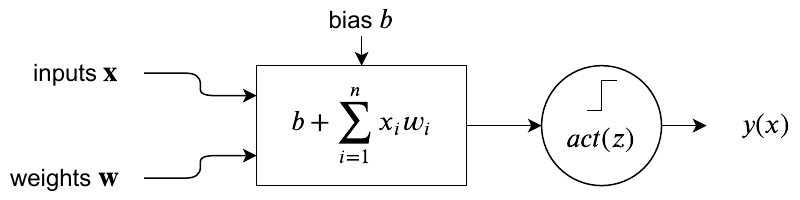
\includegraphics[width=8cm, keepaspectratio]{img/2_2_perceptron.png}
	\caption{Schematic view of the perceptron.}
\end{figure}

This definition is inspired by biological neurons and their electrophysiology: they receive some inputs, combine them and then, through the equivalent of the activation function, decide whether or not to propagate the signal \cite{Rosenblatt58theperceptron}.

\subsubsection{Deep Neural Networks}
Like in the animal brains, we can achieve interesting flexibility of the model when we link multiple perceptrons together.
In particular, during the years the community started following the approach of structuring the NNs in a layered fashion \cite{layered_nets} although, in the recent years, researchers are exploring new ways of optimizing and structuring differently the NNs to gain in performance \cite{lottery_ticket} \cite{weight_agnostic}.

\begin{figure}[H]
	\centering
	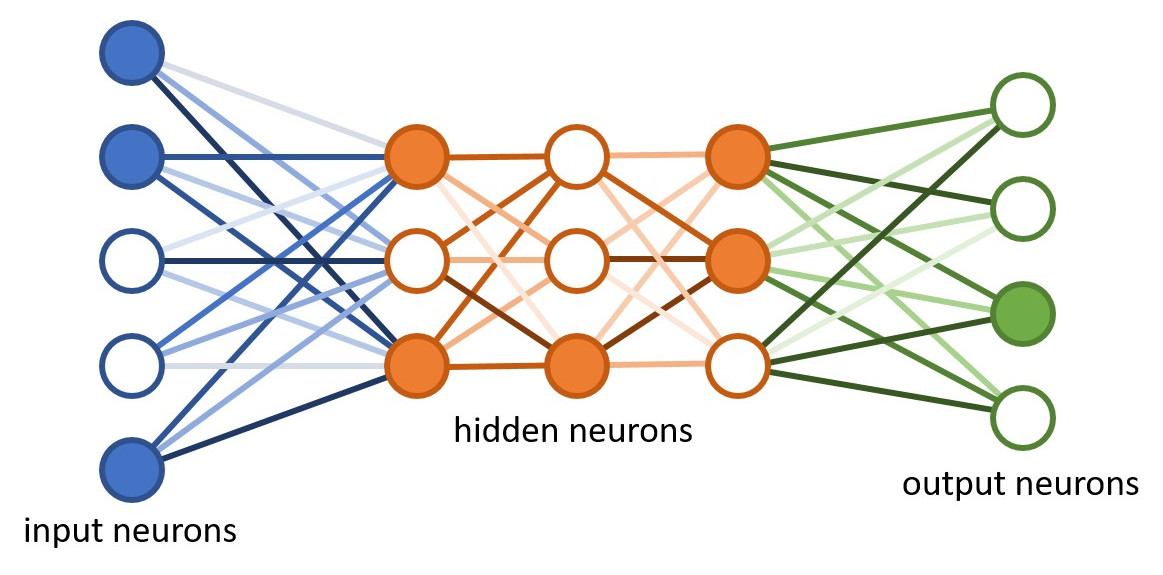
\includegraphics[width=12cm, keepaspectratio]{img/2_2_dnn.jpeg}
	\caption{Schematic representation of a Deep Neural Network ans its layers.}
\end{figure}

What makes a neural network "deep" is actually the number of layers between the \textit{input layer} and the \textit{output layer} of the network.
These layers are called \textit{hidden}.
In a layered NN, the outputs of the previous layer are the inputs to the next layer.
With the exception of a few more sophisticated structures, NNs usually form an acyclic graph, known as \textit{feed-forward network}.

It can be proven that a NN is a \textit{universal approximator} of functions \cite{hornik1989multilayer}, this means that it is possible to approximate with arbitrary precision any measurable function depending on the number of neurons present in the NN.
It is worth mentioning that choosing a \textit{non-linear activation function} allows the NN to approximate even \textit{non-linear} behaviours.
This is usually a common practice, especially when using DNN.

\subsubsection{Training of a Neural Network}
What makes the NNs so relevant is the learning procedure that is used to train them.
The vast majority of the NNs, in fact, make use of \textit{supervised learning} \cite{liu2017survey} in order to adjust the internal parameters and, therefore, learn to approximate a given function.
The term "supervised" means that the model learns being exposed to many labelled examples.
For instance, let $D$ be a training set $\{(\Bar{x}_1, y_1), \dots, (\Bar{x}_n, y_n)\}$ of arbitrary length $n$.
Each element of the set is composed of a feature vector $\Bar{x}_i$ and the respective label $y_i$.
The training procedure allows a generic NN to learn the underlying structure that links the input to the output, in the case of the training set $D$, how to map each feature vector $\Bar{x}_i$ to the respective label $y_i$.

As an example, let $f$ be a NN with one layer only, a function of the input vector $\textbf{x}$ and the matrix of its weights $\textbf{W}$ that gives us, as output, the predicted values.
The vector notation for NNs naturally extends the one of a single perceptron:
$$ f(\textbf{x}, \textbf{W}) = act(\textbf{W} \textbf{x}) $$

Let us take a generic training dataset composed by row vectors $\textbf{x}_i$ of predictors and the respective vector $\textbf{y}_i$ of the dependent variables.
Since we are in the context of \textit{supervised learning}, once the full training is completed, we would expect that our neural network has learnt how to map $\textbf{x}$ to $\textbf{y}$.
Let us provide our NN $f$ the training example $\textbf{x}$, we obtain the predicted value $\hat{\textbf{y}}$:
$$ f(\textbf{x}, \textbf{W}) = \hat{\textbf{y}} $$

We initialize the weights $\textbf{W}$ of the NN randomly and, therefore, the predicted $\hat{\textbf{y}}$ will not be very close to the desired value $\textbf{y}$.
The training procedure tunes the internal weights $\textbf{W}$ in such a way to make the predicted value $\hat{\textbf{y}}$ as close as possible to the true label $\textbf{y}$.

We introduce the concept of \textit{loss function}, that is a measure of the difference between $\textbf{y}$ and $\hat{\textbf{y}}$ or, in other words, the prediction error of the NN.
An common example of \textit{loss function} is the \textit{Mean Squared Error}:
$$ \mathscr{L}(\textbf{y}, f(\textbf{x}, \textbf{W})) =
\mathscr{L}(\textbf{y}, \hat{\textbf{y}}|\textbf{W}) =
\frac{1}{n} \sum_{i=1}^{n} (\textbf{y}_i - \hat{\textbf{y}}_i)^2 $$

$\mathscr{L}$ depends on the weights $\textbf{W}$ of the NN, therefore we can minimize it w.r.t. the weights $\textbf{W}$ and find the optimal ones for the provided training examples.
Minimizing such \textit{loss function} is not easy due to the high dimensionality of the problem and the underlying high non-linearity.
The standard procedure that set a turning point in the world of NNs and that helps to solve efficiently this problem is called \textbf{backpropagation} \cite{Rumelhart1986}.

The backpropagation algorithm computes, for each unit of the NN, the derivative of the error with respect to the weights $ \frac{\partial \mathscr{L}}{\partial w_{ij}} $ in order to come up with the \textit{gradient} of the error.
Once the \textit{gradient} has been computed, we use an \textit{optimization algorithm} that minimizes the error and updates the weights of the NN accordingly.
A very common example of \textit{optimizer} is \textbf{Stochastic Gradient Descent}, which searches for the optimal parameters in the directions where the \textit{gradient} is lower.
The stochasticity is used to add noise to the trajectory and to avoid getting stuck into a local minima \cite{zhang2004sgd}. 

The training procedure is repeated until the NN reaches the desired performances.


\subsection{Zero-sum games}
Before analyzing a GAN, we should first introduce some concepts borrowed from Game Theory useful in games with \textit{non-cooperative} setting.
The term "adversarial" comes, in fact, from the peculiar competitive interaction that takes place inside GANs' architecture.
In a non-cooperative settings with two players, for instance, a zero-sum game is a kind of game in which, whenever a player wins an specific amount the other player looses the same amount.
Basically players can only steal each others' reward, this is the reason behind the expression \textit{zero-sum}.

This concept is fundamental because it states that there's no other way of maximizing the individual gain without penalizing the other player.
Othewise, in the case of a \textit{non-zero-sum game},  players would not be forced to to overcome the opponent anymore and it would be possible to find other kind of strategies to increase the individual gain.
Instead, it is fundamental, in the context of GANs, that we keep the setting competitive.

Coming back to the \textit{zero-sum games}, the best winning strategy for each player is to apply the \textbf{minimax} strategy.
Let $V$ be the \textit{value function} that computes the expected reward given the choices of the players $a$ and $b$, we define the maximum loss as the $ \inf \{V(a,b)\}$.
The objective of both the players becomes the\textit{mini}mization of the \textit{max}imum loss.
In particular, the strategy of a player $a$ playing against $b$ is:
$$ \underset{a}{\text{min}} \; \underset{b}{\text{max}} \; V(a,b) $$

If both players played according to the minimax strategy, they would end up in a stable state of their choice: the choice of each player would no longer depend on the opponent's choice since the optimal strategy would have been found and any change to this choice would not improve the payoff.
This situation happens because, being a \textit{zero-sum game}, the best strategy is to choose the action the maximizes the personal reward assuming that the opponent is playing at its best.
This peculiar situation in which the dominant strategy is found by the two players, it is called \textit{Nash equilibrium}.

As we will see, this is a core concept for a GAN.


\subsection{Description of a GAN}
GAN architecture is composed by two NNs that play against each other in a zero-sum game \cite{gan_2014}.

The typical terminology used in GANs refers to the two architecture's NNs naming them \textbf{generator} and \textbf{discriminator}.

The \textbf{generator} is a NN $G(\textbf{z}, \theta_G)$ where $\theta_G$ indicates the network's parameters and $\textbf{z}$ is a noise vector drawn from a given prior distribution $P_z$.
$G$ is a \textit{generative model} that tries to learn the mapping between $P_z$ and the distribution $P_G$ learnt from the data distribution $P_{data}$.
The output of $G$, given $z \sim P_z$, is a sample of the distribution $P_G$.
This sample, coming from the estimated distribution $P_G$, will resemble the samples drawn from the data distribution $P_{data}$.

The \textbf{discriminator} is a NN $D(\textbf{x}, \theta_D)$ where $\theta_D$indicates the network's parameters and $\textbf{x}$ is a vector of data.
$D$ is a \textit{classifier} that outputs the probability for the vector $\textbf{x}$ to come from the training distribution $P_{data}$ or from the learnt distribution $P_G$.

\begin{figure}[H]
	\centering
	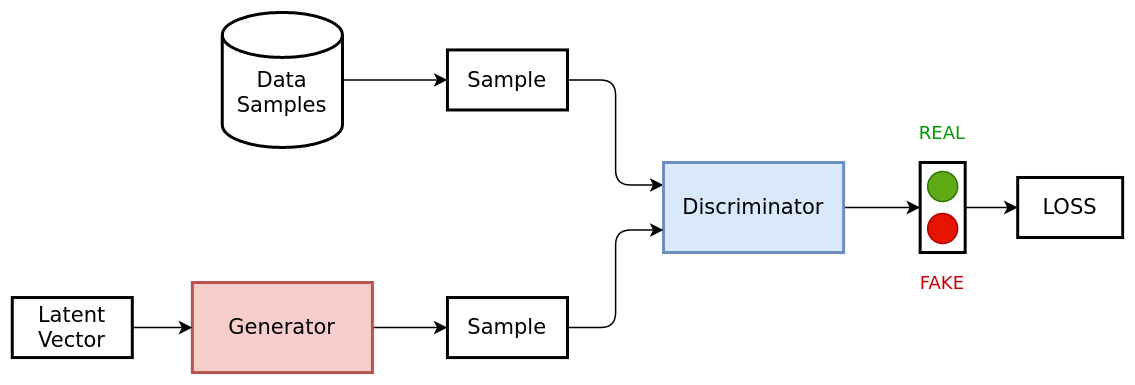
\includegraphics[width=12cm, keepaspectratio]{img/2_2_gan_arch.png}
	\caption{Schematic architecture of a GAN.}
\end{figure}

It should be clear by now that the two networks of the GAN have opposing roles.
The aim of the \textit{generator} is to produce data samples that resemble the true data distribution and, consequently, to fool the \textit{discriminator} leading it to a \textit{false-positive} classification.
On the other hand, the aim of the \textit{discriminator} that of classifying correctly as much data vectors as possible.
The two NNs are bound to this non-cooperative zero-sum game by the following \textbf{minimax} game:
$$ \underset{G}{\min} \; \underset{D}{\max} \; V(G,D) = \mathbb{E}_{x\sim p(x)}\big[\log(D(x))\big] + \mathbb{E}_{z\sim p_{z}(z)}\big[\log(1-D(G(z)))\big] $$

From the formula we can observe how $D$ tries to maximize the number of correct classifications of the original data -- the part $\log(D(x))$ -- and the generated data -- the part $\log(1-D(G(z)))$ -- while $G$, on the other hand, by tuning its internal parameters $\theta_G$, tries to minimize the number of correctly classified fake images producing more likely results.
From the formula above it is possible to derive the individual \textit{loss functions} that can be adapted to the specific problem's domain \cite{gan_loss_survery}.

Both the NNs are trained in turns and, when one NN is learning, the parameters of the other are kept constant.
Both training procedures take place as described above: starting from the \textit{loss function}, the \textit{gradient} is computed through \textit{backpropagation} and the network's weights are updated by the \textit{optimizer}.

Theoretically, after the training, the two NNs should reach the \textit{equilibrium} so that the \textit{generator} should be able to precisely mimic the data distribution $P_{data}$ and the \textit{discriminator} would guess randomly whether the presented sample is fake or not.

\subsection{Usage of GANs}
The GANs have been considered one of the most innovative idea in the field of DNNs.
Nowadays, they have many applications, especially where image manipulation is involved.
GANs, in fact, are particularly successful in the task of generating or modifying images.
For this reason GANs are usually associated with \textbf{Convolutional} NNs, a particular architecture of NN that is effective in dealing with images \cite{dcgan}.

\begin{figure}[H]
	\centering
	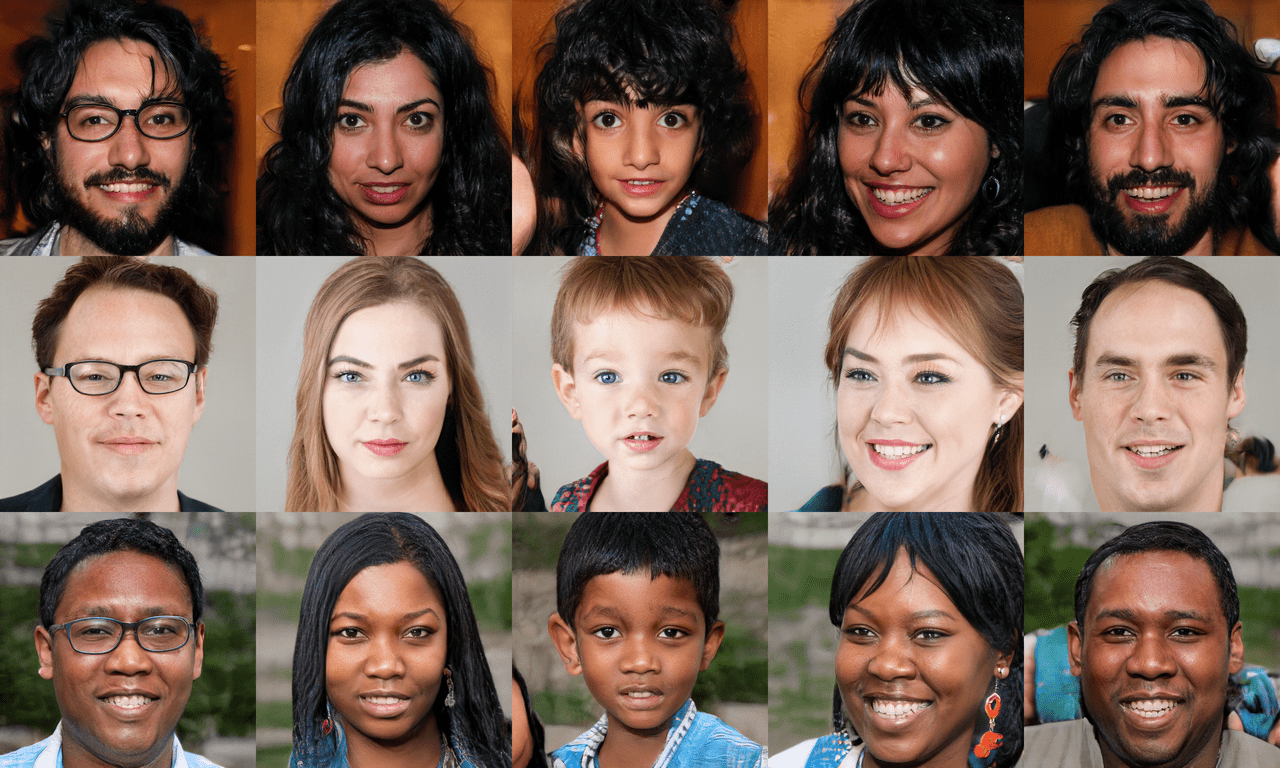
\includegraphics[width=12cm, keepaspectratio]{img/2_2_stylegan_faces.png}
	\caption{The faces above are artificially generated by StyleGAN.}
\end{figure}

Some innovative applications include:

\begin{itemize}
  \item Image super-resolution \cite{superres}, to increase the resolution and details of low resolution images
  \item Image inpainting \cite{inpainting}, to reconstruct masked/missing parts of one image
  \item Paint to image \cite{paintimg}, from a sketch or a simple paint they can reconstruct a picture
  \item Data synthesis \cite{datasynth}, used to produce synthetic samples of images similar to the ones of the training set
  \item Style transfer \cite{CycleGAN2017}, used to apply to a picture the artistic style of a given drawing
  \item Image harmonization \cite{harmonization}, to blend seamlessly two images or parts of them
\end{itemize}

\begin{figure}[H]
	\centering
	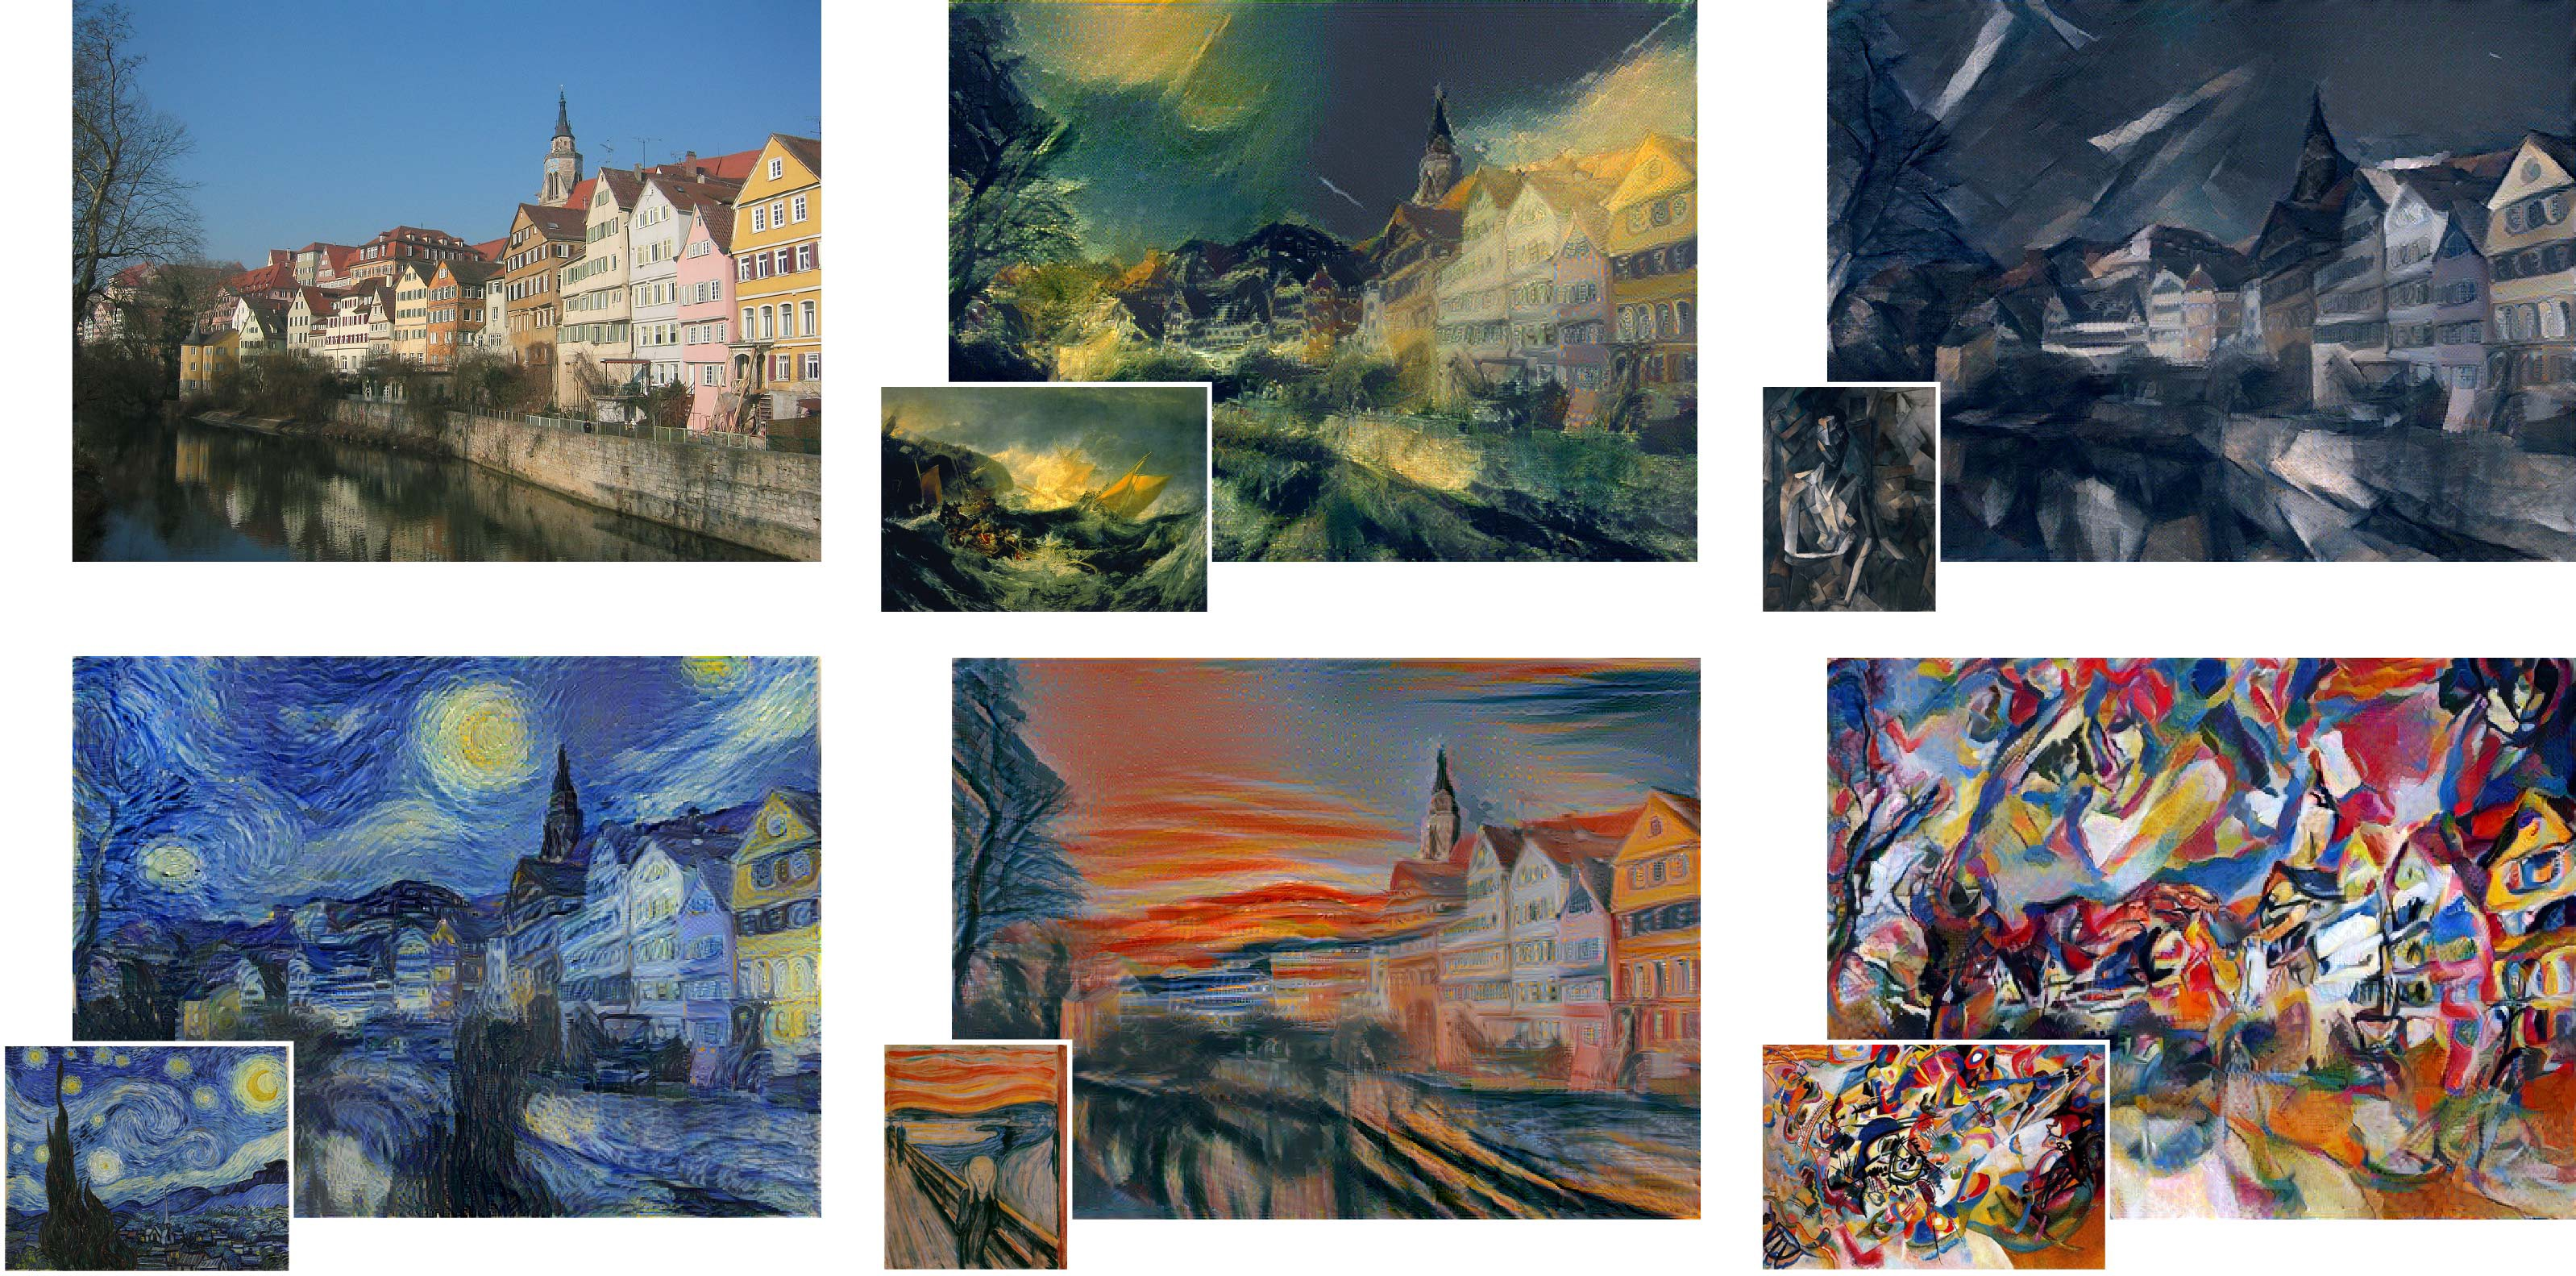
\includegraphics[width=12cm, keepaspectratio]{img/2_2_styletransfer_paintings.jpeg}
	\caption{Examples of Neural Style Transfer: a GAN trained to extract the stylistic features of paintings to apply them on pictures.}
\end{figure}

This was just a quick overview of the most promising applications of the GANs.
The research area around them is very vivid and in rapid evolution.
The power and the credibility of such technologies became so high that they started to rise some concerns due to malicious and immoderate usage \cite{tolosana2020deepfakes}.

\section{Signal Temporal Logic}

\textit{Temporal Logic} (TL) is mostly known for the formal verification of models, both hardware and software.
It was conceived to check a discrete signal measured over time against a logical proposition that makes use of special operators.

The term \textit{Temporal Logic} refers to a broad family of logics used for formal verification.
Each temporal logic follows precise rules on how to build the propositions using the allowed operators.
The aim is to analyze and check some requirements for a given \textit{time series}.
TL relies on a basic set of \textit{temporal operators} used to deal with time-related variables \cite{sep-logic-temporal}.
They are used in formal verification to assign a \textit{truth value} to a given \textit{time series} according to the properties expressed by the TL statement.

We are going to cover in detail only one kind of \textit{Temporal Logic}, the \textbf{Signal Temporal Logic} (STL).
This logic has been created to deal with continuous-time signals by discretizing them \cite{stl2004}.

\subsection{Syntax}
The basic component of a STL statement is the \textbf{atomic predicate}, generally named $\mu$.
Let $s$ be a generic signal over time $t$, an \textit{atomic predicate} $\mu$ is a logical function of the signal, i.e. $\mu = f(s(t)) > 0$ where $f$ is a generic function defined over the signal's state space $\mathcal{S}$, $f: \mathcal{S} \to \mathbb{R}$ .

STL syntax allows to chain multiple atomic predicates by means of the \textbf{operators} to obtain a STL proposition, generically referred to as $\varphi$.
The operators defined in STL are \textit{logical} or \textit{temporal}.
\textit{Logical operators} are the very same used in every logic: negation $\neg$, and $\wedge$, or $\vee$.

The \textbf{temporal operators} are introduced specifically in TLs and are used to check properties of the signal over time.
The \textit{temporal operators} defined in the STL syntax are: $\mathcal{G}$\textit{lobally}, $\mathcal{F}$\textit{inally} and $\mathcal{U}$\textit{ntil}.
The operator is referred to as \textit{bounded} if it is defined over a finite \textit{interval}, otherwise it is \textit{unbounded}.

An \textbf{interval}defines the time window in which a given operator is applied.
For instance, the notation $[0,H]$ denotes all the possible intervals $(t_i, \dots, t_{i+H})$ in the time $t = (t_0, t_1, \dots, t_n)$ over which the signal $s$ is defined.
The operator paired with a specific interval operates on the specified sliding window.
Sometimes we refer to $\mathcal{I}$ as the generic interval $\mathcal{I} = [a,b]$.

The notation for specifying a \textit{bounded operator} over the proposition $\varphi$ is, for instance, $\mathcal{G}_{[a,b]}\varphi$.
These operators specify how the given condition $\varphi$ should be evaluated with respect to the timeframe specified by the interval $[a,b]$.

Giving an intuitive explanation of the three operators:
\begin{itemize}
  \item $\mathcal{G}_{[a,b]}\varphi$: $\varphi$ must always be true within $[a,b]$
  \item $\mathcal{F}_{[a,b]}\varphi$: $\varphi$ must become true at least once within $[a,b]$
  \item $\varphi_1\mathcal{U}_{[a,b]}\varphi_2$: $\varphi_2$ must become true
at least once within $[a,b]$ and $\varphi_1$ must be always
true prior to that time
\end{itemize}

The rules of the grammar STL uses to create any formula $\varphi$ can be encoded in a very compact way:
$$ \varphi := \top \;|\; \mu \;|\; \neg\varphi \;|\;
\varphi_1 \lor \varphi_2 \;|\; \varphi_1 \mathcal{U}_{[a,b]} \varphi_2 $$

From the operator $\mathcal{U}$, it is possible to derive the other two operators, $\mathcal{F}$ and $\mathcal{G}$:
$$ \mathcal{F}_{[a,b]}\varphi = \top \mathcal{U}_{[a,b]}\varphi
\qquad \text{and} \qquad
\mathcal{G}_{[a,b]} = \neg\mathcal{F}_{[a,b]}\neg\varphi $$


\subsection{Boolean semantics}
Given the STL syntax, we can give a specific meaning to each symbol.
As we already said, the temporal logics have been created to \textit{verify} some properties and, in case of STL, signals.
The term "verification" implies the computation of a \textit{truth value}, in fact, the most natural semantics that a STL formula can have is the \textbf{Boolean semantics}.

Let $s$ be the signal defined over time $t$ and let $\varphi$ be a STL statement built to express a requirement on $s$.
The \textit{Boolean semantics} allows to \textit{check} whether a given signal $s(t)$ satisfies or not the requirements expressed by the STL proposition $\varphi$.
The satisfaction of the formula $\varphi$ is expressed by the \textit{truth value} assigned by the semantics to the specific signal $s(t)$.

It is possible to define recursively the \textit{Boolean semantics} of STL:
\begin{align*} % notation from https://arts.units.it/retrieve/handle/11368/2856192/69577/RV15-post.pdf
 (s,t) \models \mu \iff & f(s(t)) = 1 \\
 (s,t) \models \neg \varphi \iff & (s,t) \not\models \varphi \\
 (s,t) \models \varphi_1 \vee \varphi_2 \iff & (s,t) \models \varphi_1 \;\text{or}\; (s,t) \models \varphi_2 \\
 (s,t) \models \varphi_1 \mathcal{U}_{[a,b]} \varphi_2 \iff & \exists t' \in [t+a, t+b] \;\text{s.t.}\; (s,t') \models \varphi_2 \\
 & \text{and}\; \forall t'' \in [t, t'], (s,t'') \models \varphi_1
\end{align*}

The trace $s$ satisfies $\varphi$ if and only if $(s, 0) \models \varphi$.
Starting from the definition of the $\mathcal{U}$ntil operator, as we already mentioned, it is possible to derive the operators $\mathcal{F}$inally and $\mathcal{G}$lobally.

By adding these basic operations to the usual Boolean logic, we obtain the full power of the STL Boolean semantics.
With this semantics it is already possible to monitor a signal to perform verification on it.

\subsection{Quantitative semantics}
Another interesting property of STL is the possibility of attributing different semantics to the same syntax.
A \textbf{quantitative} or \textbf{robust} semantics has been formalized as well \cite{robuststl}.

This semantics uses the same notation and operators of the \textit{Boolean semantics}, but provides a different interpretation of the same formulas.
Let us introduce a function $R$ that given the triplet $(s, t, \varphi)$, computes the \textit{robustness} of the signal $s$ with respect to the proposition $\varphi$.
It is possible to define recursively how the semantics works:
\begin{align*} % notation from https://arxiv.org/pdf/1808.03315.pdf
R(s,t,(f(s) \sim \mu)) = & \begin{cases} \mu-f(s_t) & \sim=\le \\ f(s_t)-\mu & \sim=\ge \end{cases}
\\
R(s,t,\neg \varphi,t) = & -R(s,t,\varphi)
\\
R(s,t,\varphi_1 \vee \varphi_2) = & \max(R(s,\varphi_1,t),R(s,\varphi_2,t) )
\\
R(s,t,\varphi_1 \wedge \varphi_2) = & \min(R(s,\varphi_1,t),R(s,\varphi_2,t) )
\\
R(s,t,\varphi_1 \mathcal{U}_I \varphi_2) = & \underset{t^\prime \in t+I} \max \big (  
 R(s,t,\varphi_2,t'), \underset{t'' \in [t,t']} \min R(s,\varphi_1,t'')\big)
\\
R(s,t, \mathcal{F}_I \varphi) = & \underset{t' \in t+I}\max ~ R(s,\varphi,t') \\
R(s,t,\mathcal{G}_I \varphi) = & \underset{t' \in t+I}\min~  R(s,\varphi,t')
\end{align*}
The \textit{Boolean} and \textit{robust} semantics are tightly related: $R(s,t, \varphi) > 0 \iff (s,t) \models \varphi$ and $R(s,t, \varphi) < 0 \iff (s,t) \not\models \varphi$.

The intuitive idea behind the quantitative semantics is to measure the relative offset between the signal and the given requirement.
This offset represent how much the signal can be shifted before incurring into the change of the truth value for the proposition $\varphi$ and, therefore, into the violation of the constraint.
The \textit{robustness} quantify, in fact, how much variation can be tolerated on the signal.
This property of the semantics makes it particularly suitable for this work.
We are going to use it to measure the \textbf{robustness} of the trajectories proposed by our method.


\begin{figure}[H]
	\centering
	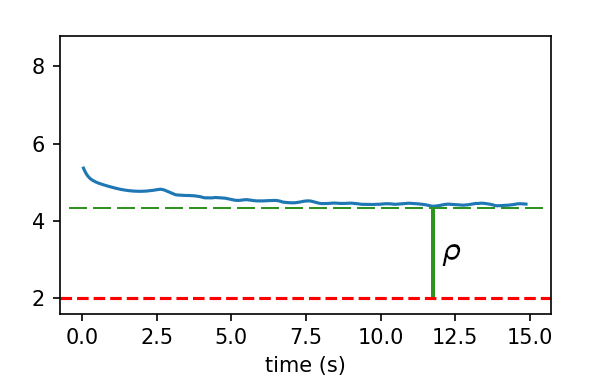
\includegraphics[width=8cm, keepaspectratio]{img/2_3_stl_robustness.png}
	\caption{The quantitative semantics of STL visualized. Let $s$ be the blue signal in the picture and let $\varphi: \mathcal{G}(s > 2)$ be the STL formula that we want to check on it, whose boundary is depicted in red. The robustness $\rho$ represents the offset between the signal and the constraint $\varphi$.}
\end{figure}
	\chapter{Method}

\section{Description}
The intuition behind the proposed method is to use GAN architectural design to automatically train a controller without providing anything but STL specifications of controller's targets and, at the same time, to obtain a generative model capable of generating difficult tests.
Our solution to such problem presents some similarities with classical GANs.
The main difference is that our \textit{generator} does not try to fool a classification performed by the \textit{discriminator}.
Our architecture is composed of two players that, in a turn-based game, try to overcome each other.

Each player is represented by a NN and the aim is to teach to one of the two NNs, referred to as \textbf{defender}, how to safely face the opponent NN, referred to as \textbf{attacker}.
Basically, the \textit{defender} tries to satisfy an STL requirement $\Phi$, while the \textit{attacker} tries to generate environmental configurations that can lead the opponent toward a violation of such requirement.

The method's achievements are twofold: on one hand we obtain a \textit{defender} able to act safely under adverse conditions, whereas, on the other hand, we obtain an \textit{attacker} able to gain some insights on the scenarios that are troubling for the \textit{defender}.

The presented method is composed of two different tightly coupled parts:
\begin{itemize}
  \item the \textbf{CPS architecture}, used to run simulations and to estimate the robustness of trajectories generated through them,
  \item the \textbf{Controller-Environment architecture} which is composed of a \textbf{defender}, which acts as a \textit{controller}, and of an \textbf{attacker}, which acts as the \textit{environment}. Both the \textit{controller} and the \textit{environment} manipulate the inputs and the outputs of the \textit{CPS architecture}.
\end{itemize}

\subsection{CPS architecture}
The \textit{CPS architecture} is represented by a model $\mathcal{M}$ that captures the dynamics of the addressed system along with its complexity.

Each model $\mathcal{M}$ is composed of a physical component whose continuous behaviour, modelled through differential equations, describes how the whole system evolves in time.
The \textit{controller} collects data from the physical world through its \textit{sensors} and decides the best action based on the evolution governed by the differential equations.

We can decompose $\mathcal{M}$ in two subcomponents:
\begin{itemize}
  \item the \textbf{agent}, denoted by $\alpha$, is the part of the system that can be controlled. In CPS terms we can think about it as the \textit{plant} that, through \textit{sensors} and \textit{actuators}, is governed by a \textit{controller},
  \item the \textbf{environment}, denoted by $\beta$, is essentially what surrounds the \textit{agent} and it cannot be controlled.
\end{itemize}

\begin{figure}[H]
	\centering
	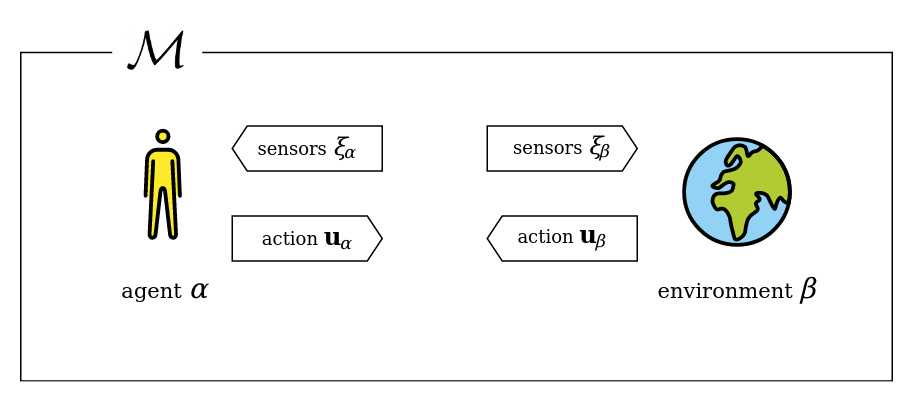
\includegraphics[width=12cm, keepaspectratio]{img/3_1_model.png.png}
	\caption{The model $\mathcal{M}$ and its components.}
\end{figure}

Let us define how this structure works.

Let $\mathcal{S}$ be the state space of dimension $m$, such that $\textbf{s} \in \mathcal{S}$ is a state of the model $\mathcal{M}$ and let $\mathcal{O}$ be the space of its observable states, having dimension $n$.
Both the \textit{agent} and the \textit{environment} can obtain full or partial information about the observable state $\textbf{o} \in \mathcal{O}$ through a series of \textit{sensors}.
We denote $\textbf{o}_\alpha \subseteq \textbf{o}$ the observable state sensed by the \textit{agent} and with $\textbf{o}_\beta \subseteq \textbf{o}$ the observable state sensed by the \textit{environment}.
Let $\xi_\alpha$ and $\xi_\beta$ be the two functions defined respectively as $\xi_\alpha: \mathcal{S} \to \mathcal{O}$ and $\xi_\beta: \mathcal{S} \to \mathcal{O}$ that, given a state $\textbf{s}$, return the observable state $\textbf{o}_\alpha$ and $\textbf{o}_\beta$.
$$ \xi_\alpha(\textbf{s}) = \textbf{o}_\alpha
\qquad \text{and} \qquad
\xi_\beta(\textbf{s}) = \textbf{o}_\beta $$

The distinction can be useful if we want to differentiate the level of the knowledge of the current state $\textbf{o}$ for $\alpha$ or $\beta$.
Such flexibility can be very useful to model specific cases of \textit{partial knowledge}.

Let $\mathcal{U}_\alpha$ be the space of dimension $l$ of all the possible actions of the \textit{agent} and let $\mathcal{U}_\beta$ be the space of dimension $r$ of all the possible actions of the \textit{environment}.
Let $\textbf{u}_\alpha \in \mathcal{U}_\alpha$ and $\textbf{u}_\beta \in \mathcal{U}_\beta$ be the actions taken.
Moreover, let $t$ be the time defined over the $\mathbb{R}$ space.
The simulator $f_\mathcal{M}$ (or simply $f$) that computes the evolution of our CPS, is defined as $f: \mathcal{S} \times \mathcal{U}_\alpha \times \mathcal{U}_\beta \times \mathbb{R} \to \mathcal{S}$ and, in particular, it is a differential equation of the form:
$$ \dot{s} = f(\textbf{s}, \textbf{u}_\alpha, \textbf{u}_\beta, t) $$

We can discretize it with respect to time $\Delta t = t_{i+1} - t_i$ and we obtain:
$$ \textbf{s}_{i+1} = \textbf{s}_i + f(\textbf{s}_i, (\textbf{u}_\alpha)_i, (\textbf{u}_\beta)_i, t_i) $$

where $i$ is the $i$-th discrete instant of time of the simulation.
We have now a discrete simulator that is able to compute the evolution of the CPS deterministically given the control actions.

Since the simulator is very dependent on the specific case study, in the next chapter we cover some examples of the equations used.

The simulator plays a crucial role: the NNs are not trained using observed examples.
Similarly to what happens in reinforcement learning \cite{reinforcementlearning}, we simply provide a simulated environment in which different choices can be made without real consequences.
This allows for a fast learning procedure that can encourage safe actions and penalize those that lead to undesired results.

In the next chapter, we describe in details how our \textit{case studies} are designed.

\subsection{Controller-Environment architecture}
The architecture is clearly inspired by that of a GAN.
In fact, we have two NNs that compete in a \textit{minimax} game for maximizing opposite goals.

The architecture is composed of:
\begin{itemize}
  \item the \textbf{attacker}, denoted by $A$, similar to a GAN \textit{generator},
  \item the \textbf{defender}, denoted by $D$, that tries to keep the CPS safe in the test scenarios.
\end{itemize}

The main difference compared to GANs is that there is no \textit{discriminator}.
The aim of the \textit{attacker} is to generate \textit{environment} configurations in which the \textit{defender} is not able to act safely, rather than trying to fool it.

Let us now describe the interaction between the physical model $\mathcal{M}$ and our adversarial NNs.
The \textit{defender} NN $D$ is the controller of the \textit{agent} in the model $\mathcal{M}$, while the \textit{attacker} is in charge of generating the worst possible configuration of the \textit{environment}.

The architecture of the two NNs can be whatever fits the problem at best.
Though, the power of the proposed approach is given by how the training is carried out, not by the NNs' design.

The two NNs produce a sequence of actions $\textbf{u}_\alpha$ and $\textbf{u}_\beta$.
Since in our approach there is no notion of time and only the state of our model $\mathcal{M}$ in a specific instant $t_i$ is known, we need our NNs to produce, for each timestep, a whole sequence of actions.
To make this possible we introduce the \textit{policy function} $\Pi_A$ for the \textit{attacker} NN e $\Pi_D$ for the \textit{defender} NN.

Let $\textbf{w}_A$ and $\textbf{w}_D$ be the coefficients' vectors defined on the spaces $\mathbb{R}^p$ and $\mathbb{R}^q$, respectively.
Let the notation $t_i \dots t_{i+h}$ denote a timeframe defined over $h$ instants.
From now on, this notation will denote sequences defined on the interval $[i, i+h]$.

The \textit{policy function} is a polynomial functions of the coefficients $\textbf{w}_i$ that produces as output a function $\textbf{u}(t)$ that, discretized as $\textbf{u}(t_i) = \textbf{u}_i $ for each timestep between $t_i$ and $t_{i+h}$, gives the sequence of actions $\textbf{u}_i \dots \textbf{u}_{i+h}$ for the considered horizon $h$.
In particular we define $\Pi_A: \mathbb{R}^p \times \mathbb{R} \to \mathcal{U}_\beta$ and $\Pi_D: \mathbb{R}^q \times \mathbb{R} \to \mathcal{U}_\alpha$ separately for each NN:
\begin{align*}
 \Pi_A(\textbf{w}_{Ai}, t)  = 
 \sum_j^p (\mathrm{w}_j)_{Ai} \cdot t^j = \textbf{u}_\beta(t)
& \quad \text{with}\quad
 \textbf{w}_{Ai} = A(\theta_A, \textbf{o}_{\beta i}, \textbf{z}_i) \\
 \Pi_D(\textbf{w}_{Di}, t)  = 
 \sum_j^q (\mathrm{w}_j)_{Di} \cdot t^j = \textbf{u}_\alpha(t)
& \quad \text{with}\quad
 \textbf{w}_{Di} = D(\theta_D, \textbf{o}_{\alpha i})
\end{align*}
The choice of the \textit{policy function} can be NN specific: for instance, they could use polynomials with different degree.

Using such \textit{policy function} has the advantage of introducing a natural smoothing and preventing an incoherent behaviour of the actions $\textbf{u}$ in two subsequent instants.

The problem of finding the best action $\textbf{u}$ has become the problem of finding the best coefficients $\textbf{w}_A$ and $\textbf{w}_D$ for the \textit{policy functions} $\Pi_A$ and $\Pi_D$.
And this is precisely the problem addressed by our NNs.
Despite the two NNs are very similar, we are going to cover them separately.

Let $\theta_A$ be the matrix of the weights and biases (the parameters) of the \textit{attacker} NN, defined on the space $\Theta_A$ of dimension dependent on NN's architecture.
As said before, the \textit{attacker} controls the \textit{environment}.
Therefore, at time $t_i$ it takes as input its own parameters $\theta_{Ai}$, the observable state $\textbf{o}_{\beta i}$ and a vector of \textit{gaussian} noise $\mathbf{z}_i \in \mathbb{R}^g$,  $\mathbf{z}_i  \sim \mathcal{N}(0, 1)$.
The introduction of such random input vector $\textbf{z}$ is borrowed from usual GANs literature: as we have seen in the previous chapter, it is possible to use this \textit{latent variable} to sample from the \textit{latent space}. 
The \textit{attacker} NN is defined as $A: \Theta_A \times \mathcal{O} \times \mathbb{R}^g \to \mathbb{R}^p$ and can be represented as the following function:
$$ A(\theta_A, \textbf{o}_{\beta i}, \textbf{z}_i) = \textbf{w}_{Ai}$$

The \textit{defender}, similarly to his opponent, controls the \textit{agent} and take as input its parameters $\theta_D$ -- the matrix of weights and biases defined over the space $\Theta_D$ of dimension dependent on NN's architecture -- and its observable state vector $\textbf{o}_{\alpha i}$.
No noise is passed as input to the \textit{defender} since there is no need to learn a distribution.
This NN must simply find the best possible set of coefficients $\textbf{w}_{Di}$.
The function is defined as $D: \Theta_D \times \mathcal{O} \to \mathbb{R}^q$ and can be represented as:
$$ D(\theta_D, \textbf{o}_{\alpha i}) =  \textbf{w}_{Di} $$

By doing so, starting from a given state of the system $\textbf{s}_i$ (from which we can observe $\textbf{o}_{\beta i}$ and $\textbf{o}_{\alpha i}$), we obtain the optimal coefficients $\textbf{w}_{Ai}$ and $\textbf{w}_{Di}$ and, by means of the \textit{policy functions}, we obtain the optimal sequence of actions $(\textbf{u}_\beta)_i \dots (\textbf{u}_\beta)_{i+h}$ and $(\textbf{u}_\alpha)_i \dots (\textbf{u}_\alpha)_{i+h}$ for the model $\mathcal{M}$ in the horizon $h$.

Given the sequences of actions in the time horizon $h$, we can now simulate via $f$ the complete evolution of the system $\mathcal{M}$.
The simulation is carried out step by step from time $t_i$ to $t_{i + h}$: at time $t_i$, a pair of actions $(\textbf{u}_\beta)_i$ and $(\textbf{u}_\alpha)_i$ is passed to $f$ that makes the system evolve into a state $\textbf{s}_{i+1}$ and so on.
Throughout the simulation we keep track of the sequence of system's states and we collect its evolution $\textbf{s}_i \dots \textbf{s}_{i + h}$.

Given the STL formula $\Phi$ for the requirement and keeping track of the sequence of the model's states $\textbf{s}_i \dots \textbf{s}_{i + h}$ evolved from the actions of both the \textit{attacker} and \textit{defender}, it is possible to compute the \textbf{robustness} of the trajectories via STL {quantitative semantics} (the function $R$ to compute the quantitative semantics has been introduced in the previous chapter):
$$ \rho_i = R(\Phi, \textbf{s}_i \dots \textbf{s}_{i + h}) $$

\begin{figure}[H]
	\centering
	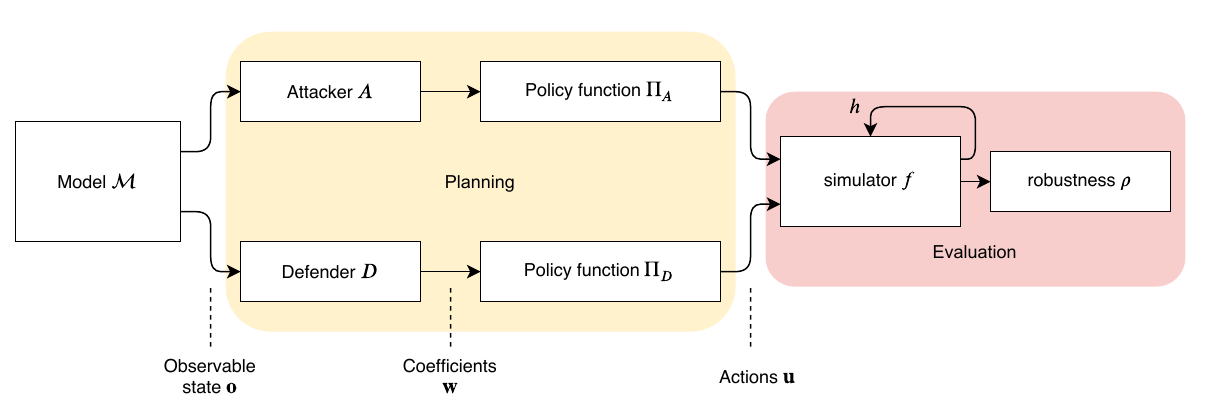
\includegraphics[width=14cm, keepaspectratio]{img/3_1_architecture.png}
	\caption{Diagram of the architecture. The model $\mathcal{M}$ observable state $\textbf{o}$ is the input of the two NNs that produce the coefficients $\textbf{w}$ for the policy functions $\Pi$. These functions gives the actions that are simulated for $h$ steps and the robustness of the system's evolution is computed.}
\end{figure}

The STL \textit{quantitative semantics}, as said in the previous chapter, measures the maximum shift that can be applied to a trajectory without varying the truth value of the requirements $\Phi$.
Therefore it is straightforward to use the \textit{robustness} $\rho$ as \textit{objective function} for tuning of the internal parameters of the NNs.

The \textit{robustness} is the quantity on which the two NNs play the \textit{minimax} game.
For convenience, let $F$ be a function $F: \mathcal{S} \times \Theta_D \times \Theta_A \to \mathcal{S}^h$ that, given a initial state $\textbf{s}_i$ of $\mathcal{M}$ and the parameters of the two NNs $\theta_D$ and $\theta_A$, computes the system's evolution in the horizon $h$:
$$ F(\textbf{s}_i, \theta_D, \theta_A) = \textbf{s}_i \dots \textbf{s}_{i+h} $$
Such function applies iteratively the simulator function $f(\textbf{s}_i, (\textbf{u}_\alpha)_i, (\textbf{u}_\beta)_i, t_i) = \textbf{s}_{i+1}$ for each pair of actions $(\textbf{u}_\alpha)_i = \Pi_D(D(\theta_D, \textbf{o}_{\alpha i}),t_i)$ and $(\textbf{u}_\beta)_i = \Pi_A(A(\theta_A, \textbf{o}_{\beta i}, \textbf{z}_i), t_i)$ computed in the interval $t_i \dots t_{i+h}$.
Then the \textit{loss function} is defined as follows:
$$ \mathscr{L}(\theta_A, \theta_D) = R(\Phi, F(\textbf{s}_i, \theta_D, \theta_A)) $$

Therefore, the \textit{minimax} game between the two is$$ \underset{\theta_A}{\min} \; \underset{\theta_D}{\max} \; \mathscr{L}(\theta_A, \theta_D) $$

In this setting, the \textit{defender} is going to tune its NN's weights in such a way to maximize the \textit{robustness} by generating safe actions for the model, while the \textit{attacker} is going to tune its NN's weights trying to generate more and more challenging scenarios for the opponent with the aim of minimizing its \textit{robustness}.


\section{Training}
The training approach borrows from the \textit{reinforcement learning} literature \cite{reinforcementlearning}.
The training is expressed as a sequence of \textbf{episodes} in which our \textit{agent} receives a feedback -- the \textit{robustness} -- for its choices and learns from it.

We define an \textit{episode} as a single safety problem to be solved.
At the beginning of each \textit{episode}, a new state $\textbf{s}_0$ of the model $\mathcal{M}$ is generated randomly to allow both the\textit{attacker} and the \textit{defender} to explore and learn from different configurations of the setting.
Then, each of them plans a strategy for the time horizon $h$, the whole evolution is simulated through $F$, and the \textit{robustness} of the specific sequence of choices is then computed in order to optimize the weights of the NNs.

Since the NNs do not take into account the past history of the opponents' actions and base the predictions solely on the current state $\textbf{s}_i$, it is possible to imagine each instant of the evolution of the system as a separate problem to solve.
This specific property that does not make any assumption on the system's evolution, allows to deal with problems using a simple architecture.
However, to explore reasonably well all the state space $\mathcal{S}$, it requires a specific kind of training in order to avoid undefined behaviours due to completely unexplored scenarios.

Due to this architecture's characteristic, in fact, it is compulsory to sample from the entire state space $\mathcal{S}$ in order to expose the NNs even to the less probable cases.
The \textit{hyper-grid} -- on which all the possible states lie -- is explored randomly adding some noise drawn from a normal distribution $\mathcal{N}(\mu, \sigma)$ where $\mu$ and $\sigma$ are respectively the mean and the variance specified according to the case study in order to maximize the diversity of the samples even in case of repeatedly sampled states.

For every sample drawn from the state space $\mathcal{S}$, a training \textit{episode} for a specific NN takes place.
The training, in fact, happens in a turn-based scheme where, both NNs make a choice but only one of them learns from that \textit{episode}.

For instance, suppose we are training $D$ at time $t_0$ and suppose we sample a state $\textbf{s}_0$, the parameters $\theta_A$ of the other NN remain constant for the specific \textit{episode}.
The following operations take place for each \textit{episode}:
\begin{align*}
 \Pi_A(A(\overline{\theta_A}, \xi_\beta(\textbf{s}_0), \textbf{z}_0), t) & = \textbf{u}_\beta(t) \\
 \Pi_D(D(\theta_D,  \xi_\alpha(\textbf{s}_0)), t) & = \textbf{u}_\alpha(t) \\
F(\textbf{s}_i, \theta_D, \overline{\theta_A}) & = \textbf{s}_0 \dots \textbf{s}_h \\
R(\Phi,  \textbf{s}_0 \dots \textbf{s}_h) & = \rho
\end{align*}
At this stage, the \textit{robustness} value $\rho$ is used only to compute the \textit{loss function} of $D$ and, hence, the backpropagation of the gradient affects only the internal parameters of the \textit{defender}.
The training of $A$ is conducted in the very same fashion.

Each training \textit{episode} can be repeated multiple times in order to make the NN try new alternative moves in the same scenario.
This strategy encourages the \textit{exploration} of different possible outcomes.
In particular, it is possible to make each NN repeat the \textit{episodes} a variable number of times.
Such mechanism is borrowed from classical GANs and it is used to balance the game between the two NNs: sometimes the task of one NN is much simpler than the other's, therefore, it needs to be artificially balanced.
Setting a different number of repetition for each NN, hence, increases the chances of convergence and prevents a NN from outperforming the other not allowing it to learn at all. 

\begin{algorithm}[H]
\setstretch{1}
\caption{Training procedure}
\begin{algorithmic}[1]
\Procedure{TrainStep}{}
    \State $s_0 \gets$ SampleRandomState()
    \For{attacker\_repetitions} \Comment{Train $A$}
        \State $z \gets \mathcal{N}(0,1)$
        \State $w_\beta \gets A(\theta_A, \xi_\beta(s_0), z)$
        \State $w_\alpha \gets D(\theta_D, \xi_\alpha(s_0))$
        \\
        \State states := [\:]
        \State states[$0$] $\gets s_0$
        \For{$i \gets 0 \dots h-1$}
            \State $u_{\alpha i} \gets \Pi_D(w_\alpha, i)$
            \State $u_{\beta i} \gets \Pi_A(w_\beta, i)$
            \State states[$i+1$] $ \gets f(s_i, u_{\alpha i}, u_{\beta i}, t_i)$
        \EndFor
        \\
        \State $\rho \gets R(\Phi, \text{states})$ 
        \State BackPropagation($A, \rho$)
        \State UpdateWeights($A$)
    \EndFor
    \\
    \State $s_0 \gets$ SampleRandomState()
    \For{defender\_repetitions} \Comment{Train $D$}
        \State $z \gets \mathcal{N}(0,1)$
        \State $w_\beta \gets A(\theta_A, \xi_\beta(s_0), z)$
        \State $w_\alpha \gets D(\theta_D, \xi_\alpha(s_0))$
        \\
        \State states := [\:]
        \State states[$0$] $\gets s_0$
        \For{$i \gets 0 \dots h-1$}
            \State $u_{\alpha i} \gets \Pi_D(w_\alpha, i)$
            \State $u_{\beta i} \gets \Pi_A(w_\beta, i)$
            \State states[$i+1$] $ \gets f(s_i, u_{\alpha i}, u_{\beta i}, t_i)$
        \EndFor
        \\
        \State $\rho \gets R(\Phi, \text{states})$ 
        \State BackPropagation($D, \rho$)
        \State UpdateWeights($D$)
    \EndFor
\EndProcedure
\end{algorithmic}
\end{algorithm}


\section{Testing}
Once a sufficiently high number of \textit{episodes} has been completed, the two NNs are ready to be used as \textit{controller} and {test generator} of our CPS.
It is possible to use the two NNs separately: in fact, once trained, they become completely independent one from the other.

The testing phase differs slightly from the training one since, in real scenarios, we do not have \textit{episodes} but a continuous evolution of the system.
Therefore, the strategy of computing an optimal plan for the time horizon $h$ and applying it, does not fit such scenario.

We took inspiration from the \textit{Model Predictive Control} algorithm \cite{mpc} to design the application of our method: in simple words, at each timestep $t_i$, the optimal strategy over $h$ steps is computed as in the training step but, instead of passing all the actions $\textbf{u}_i \dots \textbf{u}_{i + h}$ to the simulator, we execute only the first one and, on the next iteration, the new state $\textbf{s}_{i + 1}$ is used to compute the next move.
More precisely, the following operations are repeated iteratively:
\begin{align*}
 \Pi_A(A(\overline{\theta_A}, \xi_\beta(\textbf{s}_i), \textbf{z}_i), t) & = \textbf{u}_\beta(t) \\
 \Pi_D(D(\overline{\theta_D},  \xi_\alpha(\textbf{s}_i)), t) & = \textbf{u}_\alpha(t) \\
 f(\textbf{s}_i, (\textbf{u}_\alpha)_i, (\textbf{u}_\beta)_i, t_i) & = \textbf{s}_{i + 1}
\end{align*}

Since the NNs are trained and they are not learning anymore, we marked both their parameters with an overline.

Due to the iterative scheme of the policies, the proposed method acts as a \textbf{closed-loop} CPS.
At timestep $t_i$, in fact, an action is taken with respect to the time horizon $h$ and the new state $\textbf{s}_{i+1}$ is reached.
Through the \textit{sensors}, our NNs will be able to retrieve the observed state $\textbf{o}_{i+1}$ that will be used to compute the next action.
Such iterative procedure allows to handle automatically cases in which the desired state is not fully reached due to unexpected causes: the algorithm will plan a new optimal strategy starting from the new observed states, hence taking into account the possible errors that have been made.

\begin{algorithm}[H]
\setstretch{1}
\caption{Test procedure}
\begin{algorithmic}[1]
\Procedure{Execute}{$\mathcal{M}$, timesteps}
    \For{$i \gets 0 \dots$ timesteps}
        \State $s_0 \gets$ GetState($\mathcal{M}$)
        \\
        \State $z \gets \mathcal{N}(0,1)$
        \State $w_\beta \gets A(\theta_A, \xi_\beta(s_0), z)$
        \State $w_\alpha \gets D(\theta_D, \xi_\alpha(s_0))$
        \\
        \State $u_\beta \gets \Pi_A(w_\beta, 0)$
        \State $u_\alpha \gets \Pi_D(w_\alpha, 0)$
        \\
        \State DoAction($\mathcal{M}, u_\alpha, u_\beta$)
    \EndFor
\EndProcedure
\end{algorithmic}
\end{algorithm}

	\chapter{Case study}

\section{Cruise control}
We used as a preliminary test of the architecture the \textit{cruise control} problem.
Such problem, even if it does not fully exploit the capabilities of our architecture, was selected since it is one of the classic baseline problem used as CPS.
The problem is more than half-century old and has been solved mechanically \cite{teetor1948mech_cc} at first and, finally, electronically \cite{wisner1971elect_cc} around the '70s.

The aim is very simple: to keep a vehicle running at constant velocity regardless of the \textit{steepness} of the road.
The model used, due to the nature of the problem, does not present a \textit{reactive environment} and, therefore, it does not fully exploit the potential of the our method.
The \textit{environment} of this setting is the road and its steepness that, once defined, cannot vary.

\textit{Cruise control} systems make use of specific \textit{sensors} to measure the current car velocity and one \textit{actuator}, able to vary the engine fuel intake of the engine according to the \textit{controller} decision.

\subsection{Model}
The model $\mathcal{M}$ in such scenario is composed of the \textit{agent} $\alpha$, represented by the car $c$, and the \textit{environment} $\beta$, represented by the road.

The road $r$ is static: in fact, once generated by the \textit{attacker} NN, it remains the same for entire \textit{episode}.
It is generated as a function that represents its elevation profile.
In this specific setting, we generate the road on the physical space $x$ using the \textbf{Radial Basis Function} with a \textit{Gaussian} kernel.

Let $d$ be the number of \textit{RBFs} that we want to sum to generate $r$, let $\pmb{\mu}$ be an arbitrary vector of dimension $d$ that represents the centers of the \textit{RBFs}, let $\pmb{\sigma}$ be the vector of dimension $d$ that represents scale factor of the \textit{RBFs},
let $\pmb{\omega}$ be the vector of dimension $d$ that weights the contribution of each RBF.
The function used to describe the road is:
$$ r(x) = \sum_i^d \omega_i \; \exp \left(- \frac{\lvert\lvert x - \mu_i \rvert\rvert^2}{\sigma_i^2}\right) $$
The vector $\textbf{u}_\beta$ generated by the \textit{attacker} is built such that $\textbf{u}_\beta = (\pmb{\omega}, \pmb{\sigma})$.
In this way the \textit{attacker} NN can influence the generation of the road.

At each instant, the car $c$ have knowledge of its current velocity $v_c$ and, trough some tilt sensors, it can also measure the steepness of the road in its current position $\theta_c = r'(x_c)$, where $x_c$ is the position of the car.
The car can control its acceleration $a_c$ through the actuator that controls the throttle.

Given the setting described above, it is possible to turn the requirement into a STL formula.
Since it must hold for the whole trajectory of the car, we used the $\mathcal{G}$lobally operator.
Let $\tilde{v}$ be the desired steady velocity and $\varepsilon$ be the tolerance on such value.
The STL formula for the requirement $\Phi$ is:
$$ \Phi = \mathcal{G}(v_c \geq \tilde{v} - \varepsilon \; \wedge \; v_c \leq \tilde{v} + \varepsilon) $$

Since the road's steepness is generated only once at the beginning of each \textit{episode}, the only part of the CPS that evolves in time through differential equations is the \textit{agent}'s one.
In particular, the continuous model of the \textit{agent} operates some simplifications:
\begin{itemize}
  \item it is seen as punctiform;
  \item it cannot steer.
\end{itemize}

Let $m$ be the mass of the car (can be disregarded in this case), $g$ be the gravity of $9.81 \frac{m}{s^2}$, $\nu$ be the friction constant of $0.01$.
We call $\left( \frac{dv}{dt} \right)_{in} = a_c$ the controllable acceleration that is provided to the car by the \textit{actuator}.
The car dynamics follows the differential equation:
$$ m \frac{dv}{dt} = m \left( \frac{dv}{dt} \right)_{in} - \nu mg\cos\theta_c   - mg\sin\theta_c$$

The formula above describes how the velocity varies over time.
We can see its dependency on the given acceleration $a_c$, to which we subtract the friction and the vertical component of its weight.

In this case study, the \textit{attacker} is very simple.
It does not take any input depending on the state of $\mathcal{M}$, hence the observable state $\textbf{o}_\beta = \varnothing$.
It gives as output the vector $\textbf{u}_\beta$ to build the function $r(x)$ that represents the profile of the road.
We limited the maximum steepness allowed to the interval $[-25\degree, 25\degree]$ by setting some constraints on $r'(x)$ to prevent trivial adversarial scenarios (vertical walls).

The \textit{defender}, on the other side, takes as input the observable state $\textbf{o}_\alpha = (v_c, \theta_c)$ and gives as output the acceleration $\textbf{u}_\alpha = (a_v)$ of the car $c$.
The simulated model has been limited to allow accelerations in the interval $[-3 \frac{m}{s^2}, 3 \frac{m}{s^2}]$, while the range of allowed velocities is $[-10 \frac{m}{s}, 10 \frac{m}{s}]$.

\section{Car platooning}
We selected the problem of \textit{car platooning} \cite{carplatooning} to test the full potential of our architecture.
This kind of setting is relatively new and it has been developed in the field of \textit{Autonomous Driving}.
The platooning, in fact, is the formation of a line of vehicles in which they follow each other in a controlled way: they should never hit the car in front and they should always have enough space in order to brake on time in case of sudden change of leader's speed.
This case study is starting to gather interest since it promises to reduce the cost of the transport and increase the overall transportation infrastructures' efficiency \cite{platooning_survey}.

Nowadays this problem has been faced with many composite techniques \cite{platooning_survey} to coordinate the actions of the car's pool, most of them rely on the so called \textit{vehicular ad-hoc networks} that can be of the type \textbf{V2V} (Vehicle to Vehicle) or \textbf{V2I} (Vehicle to Infrastructure).

This approach, though, requires specific hardware and a distributed system of coordination that can be an impossible requirement to meet in some cases.
Testing our approach to obtain a robust controller on this kind of problem is interesting, at it explores the possibility of an \textit{individual-basis} decision system.

\subsection{Model}
In the car platooning setting we have $n$ cars that follow each other forming a line.
Following a strategy of \textit{divide et impera}, it is possible to consider just the problem of two cars before generalizing the solution.

In the model $\mathcal{M}$, that we are going to define, we have one leader $l$ and one follower $f$.
Both leader and follower have an internal state that keeps track of the car's position $x$, velocity $v$ and acceleration $a$. 

The requirement $\Phi$ for the problem can be expressed in STL as
$$ \Phi =  \mathcal{G}(d \leq d_{max} \; \wedge \; d \geq d_{min}) $$

where $d = x_l - x_f$ is the distance between $l$ and $f$, and $d_{max}$ and $d_{min}$ are respectively the maximum and minimum distance allowed.
Such distance can be estimated or measured.
In our experiment, we assume that we can measure it by means of a \textit{LIDAR scanner}.
This kind of hardware, that makes use of a laser beam to measure distances, is already installed on some autonomous or semi-autonomous cars.

We used the operator $\mathcal{G}$lobally in the STL formula because we want the property to hold for the whole trajectory of the cars.
The minimum distance allowed was set at $2$ meters and the maximum one at $10$.

Since our aim is to have a safe controller that is able to follow the car ahead under the requirement $\Phi$, it comes natural to label the follower $f$ as the \textit{agent} $\alpha$ of our model $\mathcal{M}$, while all the rest is addressed as $\beta$, the \textit{environment}.
This definition implies that the leader $l$ is considered part of the \textit{environment} too.

Defined the roles inside our abstract model $\mathcal{M}$, we can now analyze how the underlying CPS is configured.
To describe the car's physical behaviour, we need to operate some simplifications:
\begin{itemize}
  \item they are seen as punctiform;
  \item they can move exclusively on a straight line;
  \item they move on a flat landscape;
  \item they can only move forward.
\end{itemize}

Let $\nu$ be the friction coefficient of $0.01$, $g$ be the gravity of $9.81 \frac{m}{s^2}$ and $m$ the mass (that can be disregarded in this case).
The differential equation that describe the car's dynamic is the following:
$$ m \frac{dv}{dt} = m \left( \frac{dv}{dt} \right)_{in}  - \nu mg  $$

The formula above represents the variation of the final velocity of the car with respect to time, given as input the car's acceleration  $\left( \frac{dv}{dt} \right)_{in} = a$ and subtracting the friction due to the movement.

In this specific case study, since both the \textit{agent} and the \textit{environment} are very similar, also their inputs are alike: both are single-element vectors $\textbf{u}_\alpha = (a_f)$ and $\textbf{u}_\beta = (a_l)$ that control the cars' acceleration.
$a_f$ and $a_l$ are respectively the accelerations that the \textit{agent} and the \textit{environment} are going to provide to the dynamic equation illustrated above.
To be more realistic, we limited the acceleration of the car to $[-3 \frac{m}{s^2}, 3 \frac{m}{s^2}]$ and the velocity to $[0 \frac{m}{s}, 20 \frac{m}{s}]$.

In this specific case study, moreover, $\textbf{o}_\alpha \equiv \textbf{o}_\beta$, hence we can refer to the model's state simply as $\textbf{o}$.
This vector contains information about the state of $\mathcal{M}$, in particular $\textbf{o} = (v_l, v_f, d)$, where $v_l$ is leader's velocity, $v_f$ is follower's velocity and $d$ is the relative distance.
	\chapter{Experimental results}

\section{Implementation details}
We implemented as a Python framework the whole architecture that has been described so far.

The code of the project can be divided into 3 parts.
\begin{itemize}
  \item The \textbf{model}: it contains the code of the physical model. The latter must be \textit{differentiable} and should comply with some internal API in order to be integrated effortlessly inside the rest of the library;
  \item the \textbf{NNs architecture}: it is the core of the project and it is configurable only via a defined API;
  \item the \textbf{experimental setup}: it is the code where the user can tweak all the parameters and decide how to test the chosen model.
\end{itemize}

\begin{figure}[H]
	\centering
	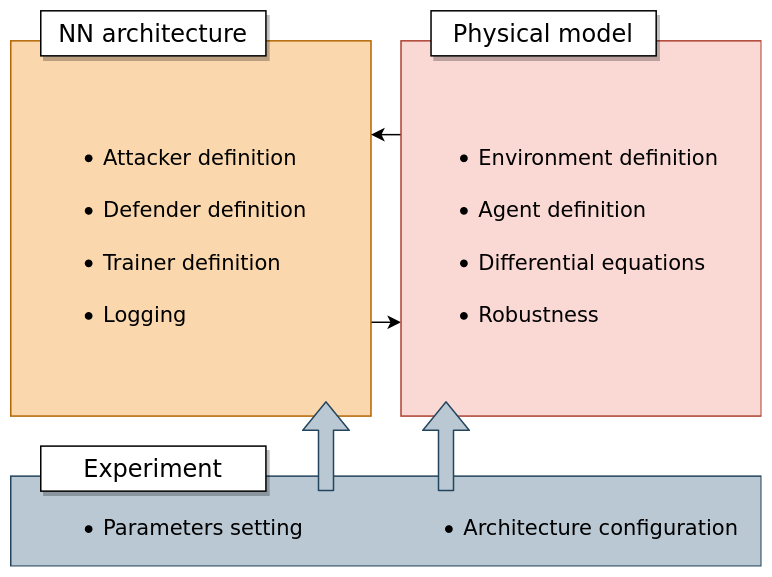
\includegraphics[width=10cm, keepaspectratio]{img/5_1_module_api.png}
	\caption{Schematic visualization of the interaction between the three main module of the architecture. The structure reflects the organization of the code as well.}
\end{figure}

In order to compute the robust semantics of the STL formulas in a fast and efficient way, it has been implemented a small separate module that parses and transforms the STL requirements into executable code.

The whole project relies extensively on PyTorch \cite{pytorch}, a Python library tailored to build complex numerical models.
All the computations leverage the PyTorch's computational graph, which eased the implementation and made the training of the NNs possible.
Unfortunately, due to the iterative nature of the training process, porting it on GPU did not provide benefits. In this regards there is room for improvements.


\section{Cruise control}
The problem of the cruise control has been described in the previous section: given a vehicle that moves along a road, the controller should be able to keep its velocity constant regardless of the steepness of the road.

\subsection{Experimental settings}
For the desired constant velocity, we fixed as \textit{setpoint} $\tilde{v} = 5 \frac{m}{s}$ and a tolerance $\varepsilon = 0.25 \frac{m}{s}$.
Therefore, the \textbf{constraint} applied to the velocity $v_c$ of the moving car $c$, is $\Phi = \mathcal{G}(v_c \leq 5.25 \wedge v_c \geq 4.75)$.

Due to the nature of the problem, the attacker controls the generation of the steepness of the road.
Such operation takes place \textbf{once}, at the beginning of each episode.

The \textbf{attacker}'s architecture has 2 layers with 10 neurons each.
To each layer is applied the \textit{Leaky ReLU} activation function \cite{xu2015empirical}.
The input noise vector $\textbf{z}$ belongs to the space $\mathbb{R}^5$.
This NN does not have other input since the \textit{environment} (the road) is a static object with no knowledge about the setting.
The output of the NN is the vector $\textbf{u}_\beta = (\pmb{\omega}, \pmb{\sigma})$ used to determine the function of the elevation of the road $r(x)$.
The dimension $d$, that defines the number of \textit{RBFs} composing $r(x)$, has been fixed to 3.

Since the environment is static and does not need to describe a dynamic behaviour, the \textit{policy function} of the attacker is defined over the space $\mathbb{R}^1$.

The \textbf{defender} NN has 3 layers with 10 neurons each.
To each layer is applied the {Leaky ReLU} activation function.

The \textit{defender} NN uses a \textit{policy function} defined over the space $\mathbb{R}^3$, due to the need of adapting and forecasting different scenarios.

The \textbf{initial configuration} of each training episode is sampled from an \textit{hyper-grid} of two dimensions: initial position $x_{c0}$ and initial velocity $v_{c0}$.
The initial position $x_{c0}$ is sampled uniformly from the interval $[0 \; m, 50 \; m]$.
Such choice has been made to introduce variability in the training and force the NNs to explore different strategies.
The initial velocity $v_{c0}$ is sampled among 25 equispaced points between $[-12 \frac{m}{s}, 12 \frac{m}{s}]$.

\begin{figure}[H]
	\centering
	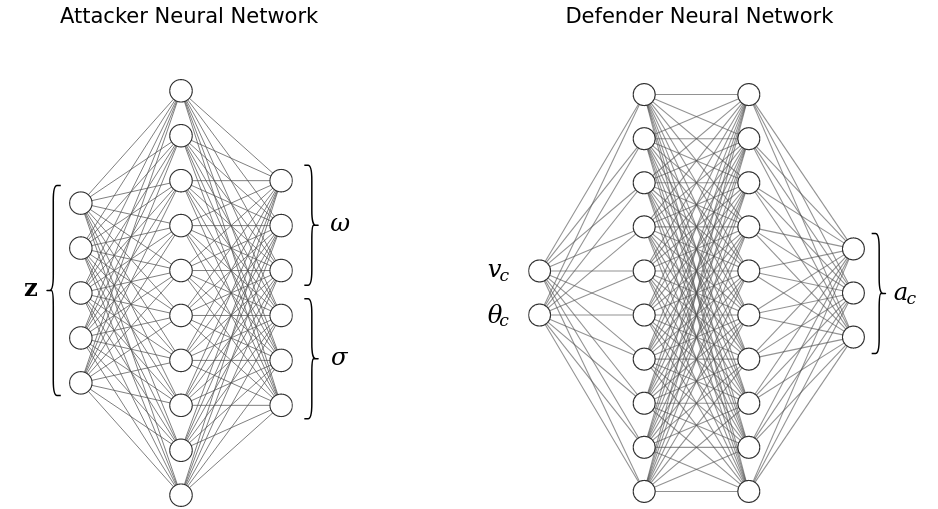
\includegraphics[width=12cm, keepaspectratio]{img/5_2_NNcruisecontrol.png}
	\caption{The architecture used for the the two NN in the cruise control case study. The \textbf{attacker} takes as input the noise vector $\textbf{z}$, while the output are the two vectors $\pmb{\omega}$ and $\pmb{\sigma}$ that characterize the . The \textbf{defender} takes as input the car's velocity $v_c$ and the inclination of the car (steepness) $\theta_c$ to compute the acceleration $a_c$.}
\end{figure}

During the training the \textbf{timestep} $\Delta t$ between two time instant has been set to $0.05s$ while the horizon $h$ for each episode was $500ms$, 10 timesteps.
The same \textit{timestep} has been used also in the testing.

The training phase lasted $30k$ \textit{cycles} and each \textbf{episode} has been repeated only 1 time for the \textit{attacker} and 10 times for the \textit{defender}.

\subsection{Metrics and results}
The testing configurations is the same of the training except for the the initial position $v_{c0}$ of the car, that is always assumed to be $0 \; m$.

We decided to test the model in three different scenarios.
In the first scenario the road is generated by the attacker NN by means of the \textit{RFBs}.
They create more complex shapes and produce realistic road profiles, this make them perfectly suitable for training but less suitable for assessing the performance of the controller.

In the second and third scenarios we have a flat landscape and, respectively, only one hill and only one valley.
Such simple tests are good to identify the pitfalls of the trained model.

In each figure we show the elevation of the road, the velocity of the car and the acceleration provided by the \textit{defender}.

\begin{figure}[H]
	\centering
	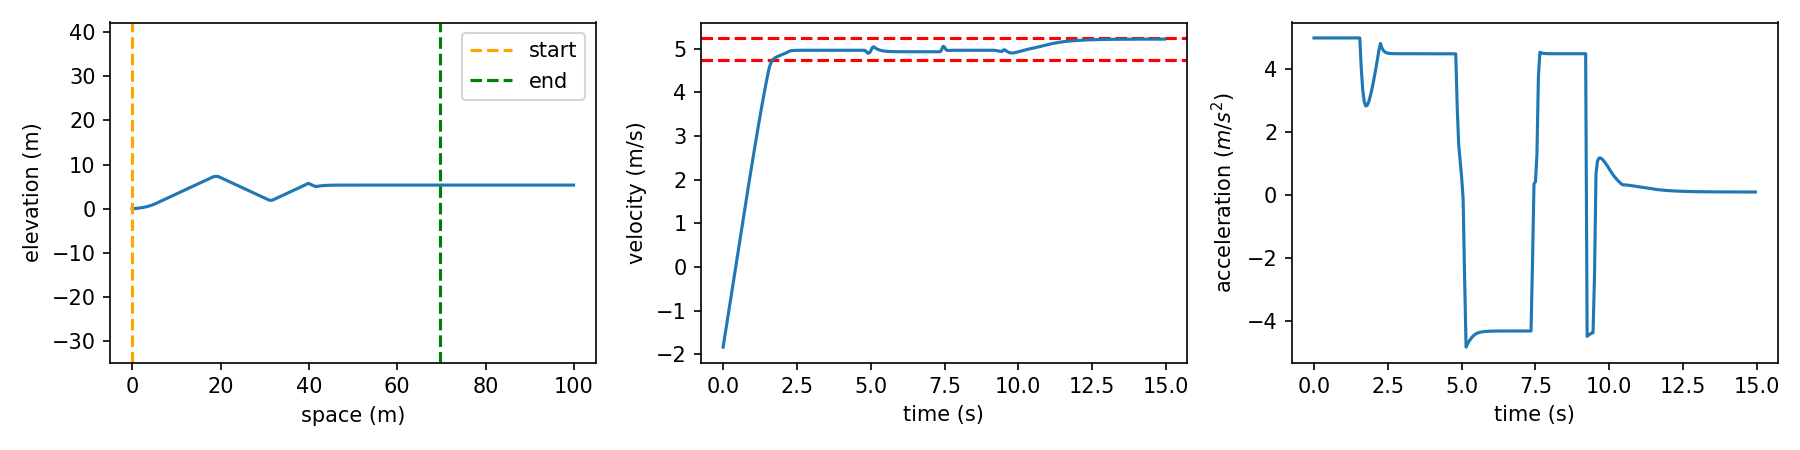
\includegraphics[width=13.8cm, keepaspectratio]{img/5_2_triplot_atk.png}
	\caption{Initial configuration: $v_{c0}=-2.04 \frac{m}{s}$. The model manages to reach the area of the desired velocity even starting from afar. Looking at the acceleration, it is possible to notice the adaptation of strategy in presence of a sudden change of steepness.}
    \label{fig:cruise_atk}
\end{figure}

\begin{figure}[H]
	\centering
	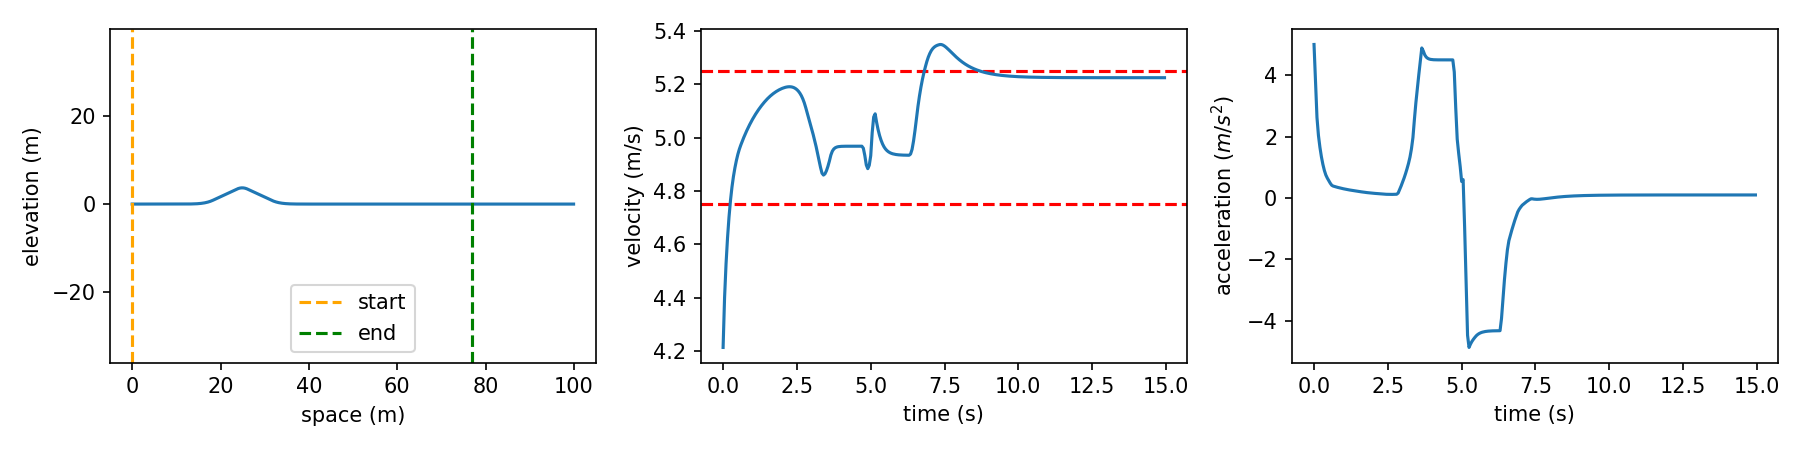
\includegraphics[width=13.8cm, keepaspectratio]{img/5_2_triplot_up.png}
	\caption{Initial configuration: $v_{c0}=3.96 \frac{m}{s}$. Here the car start with a velocity that is quite close to the setpoint. However, the trajectory presents a bit of overshoot in the correction that takes place right after the descent.}
    \label{fig:cruise_up}
\end{figure}

\begin{figure}[H]
	\centering
	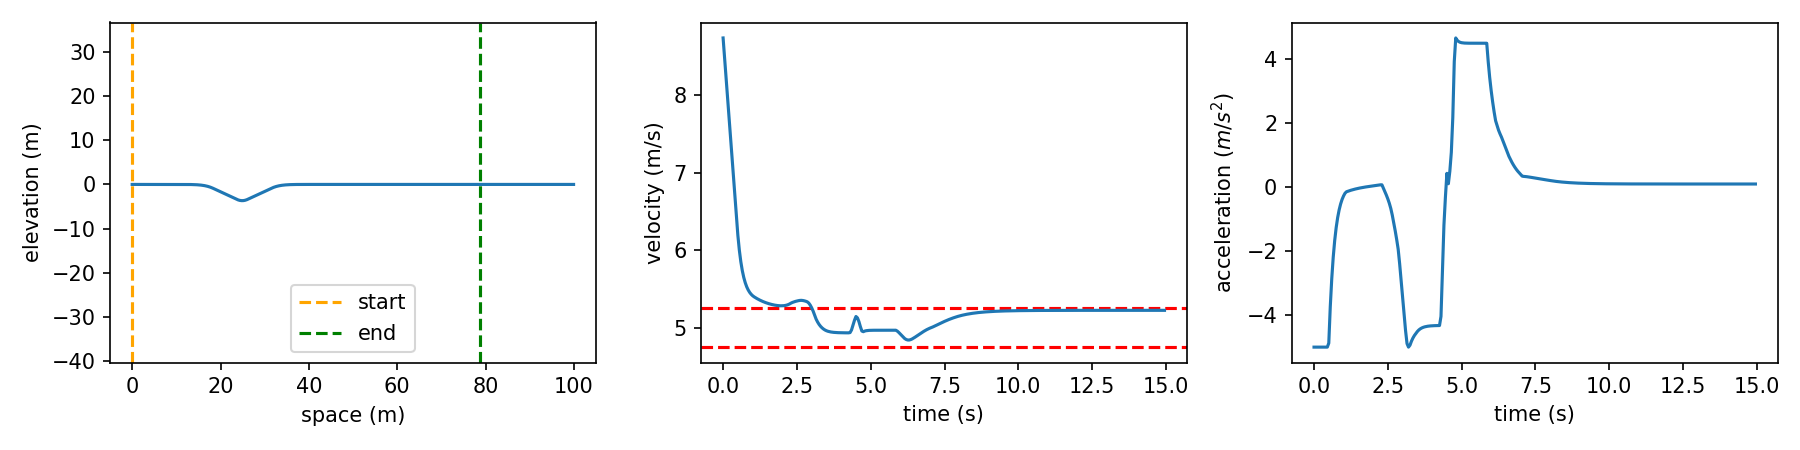
\includegraphics[width=13.8cm, keepaspectratio]{img/5_2_triplot_down.png}
	\caption{Initial configuration: $v_{c0}=8.98 \frac{m}{s}$. In such scenario we see how the defender is able to tackle two problems at the same time: reaching the setpoint and reacting to the change of slope. Still it succeed in managing the situation in a quite stable way.}
    \label{fig:cruise_down}
\end{figure}
In the figures above we can observe how different are the reaction patterns in the case of \textit{attacker}-generated scenario and artificial one.
The \textit{defender} reacts to the landscape generated by the adversarial NN, without noticeable overshoot and handles the situation in a smooth way.
In the case of the artificial hill and valley, instead, it varies more frequently the acceleration patterns even if the profile of the road is much simpler.
In every case, though, the \textit{defender} is able to rapidly reach the desired velocity and keep it. 

In order to perform model comparison and evaluate the performance of the trained model, we ran $10k$ simulations of trajectories.
The following plot shows the percentage of  trajectories that in a given instant was inside the boundary specified by the requirement.

\begin{figure}[H]
	\centering
	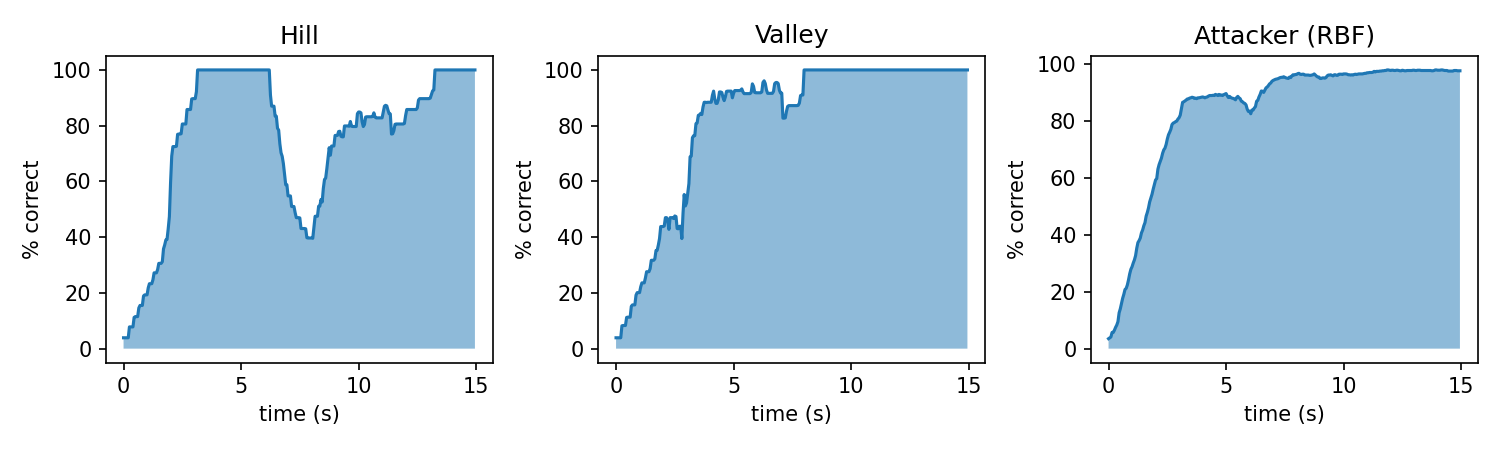
\includegraphics[width=10cm, keepaspectratio]{img/5_2_pct_histogram.png}
	\caption{This plot shows that every single trajectory simulated reached successfully the target velocity, in the end. It is possible to observe how the training on the attacker was very effective. The experience gained in such scenario, though, is less useful in the others, especially in front of sudden change of slope.}
    \label{fig:cruise_pct}
\end{figure}

In the figure \ref{fig:cruise_pct} we can see how successful was the adversarial training for the \textit{defender}: it learnt how to face every possible configuration generated from the attacker.
The smooth growth tells that it can gradually improve the situation over time until it reaches the setpoint.

The first two pictures, instead, show that there is room for improvement for the generalization ability of the \textit{defender}'s NN.
Since the result are already very promising, a better exploration of the space of the road's configuration could lead to perfect results.

\section{Car platooning}
We decided to split the problem of car platooning into a simpler problem of only two cars.
In such simplified setting, we trained both the \textit{attacker} and the \textit{defender} and finally we generalized the behaviour to $n$ cars.
We recall that the problem we want to address is the generation of a safe controller that controls the acceleration of its vehicle in order to keep the distance with the other vehicle inside a given range.

\subsection{Experimental settings}
In the simplified setting of the two cars, we have a \textit{leader} $l$ and a \textit{follower} $f$.
The \textbf{constraint} applied on the CPS described in the chapter before is on the \textit{distance} $d$ between the two vehicles and is $\Phi = \mathcal{G}(d \leq 10 \wedge d \geq 2)$.

Every \textbf{initial configuration} of the experimental runs has been sampled on an \textit{hyper-grid} of three dimensions: leader's velocity $v_{l0}$, leader's position $x_{l0}$ and follower's velocity $v_{f0}$.
The initial velocities $v_{l0}$ and $v_{f0}$ have been sampled among 40 equispaced values in the interval $[0 \frac{m}{s}, 20 \frac{m}{s}]$.
The initial leader's position $x_{l0}$ have been sampled among 15 equispaced values in the interval $[1 \; m,12 \; m]$ while the follower's $x_{f0}$ has been set to $0 \; m$.

The \textbf{attacker}'s architecture is a dense 3-layered NN with 10 neurons per layer.
To each layer has been applied the \textit{Leaky ReLU} activation function \cite{xu2015empirical}.
The dimension of the space to which the noise vector $\textbf{z}$ -- input of the \textit{attacker} NN -- belongs, has been set to $2$.
The \textbf{defender} NN has the same structure of the \textit{attacker} except for the input dimension (does not take as input a noise vector).
In order to compute the trajectory of the actions, both the NNs use a polynomial \textbf{policy function} of order 3.
Therefore, the spaces over which $\textbf{w}_A$ and $\textbf{w}_D$ are defined, have dimension $q = p = 3$.

\begin{figure}[H]
	\centering
	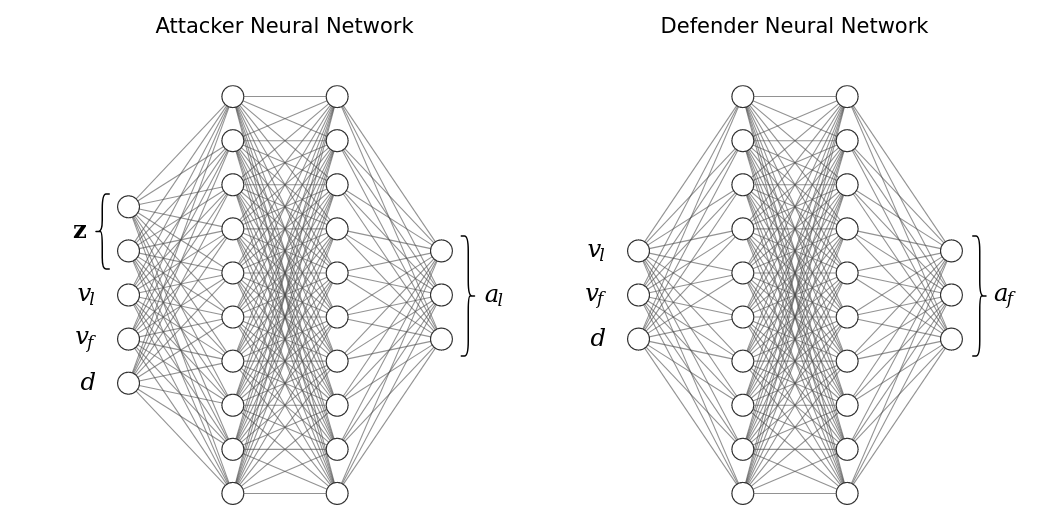
\includegraphics[width=12cm, keepaspectratio]{img/5_3_NNplatooning.png}
	\caption{The architecture used for the the two NN in the car platooning case study. The \textbf{attacker} takes as input the noise vector $\textbf{z}$, the leader's velocity $v_l$, the follower's velocity $v_f$ and their distance $d$. It gives as output the acceleration $a_l$ for the leader's car. The \textbf{defender} takes the same input of the attacker except $\textbf{z}$ and gives as output the follower's acceleration $a_f$.}
\end{figure}

During the training the \textbf{timestep} $\Delta t$ between two time instant has been set to $0.05s$ while the horizon $h$ for each episode was $5s$, 100 timesteps.
The same \textit{timestep} has been used also in the testing.

The training phase lasted $50k$ \textit{cycles} and each \textbf{episode} has been repeated 3 times for the \textit{attacker} and 5 times for the \textit{defender}.

\subsection{Metrics and results}

\subsubsection{One leader and one follower}
We tried many configuration of the hyper-parameters of the model in order to find the ones that were giving the good results presented.

We tested the \textbf{defender-controlled} follower in four different scenarios to check if it was able to adapt effectively to different adversarial strategies.
The first scenario is against the \textit{attacker}, in the second the leader accelerates suddenly, in the third the leader brakes suddenly while in the fourth it accelerates rapidly to brake right after.
For each scenario we show the position of the cars, the relative distance and the acceleration of both.

\begin{figure}[H]
	\centering
	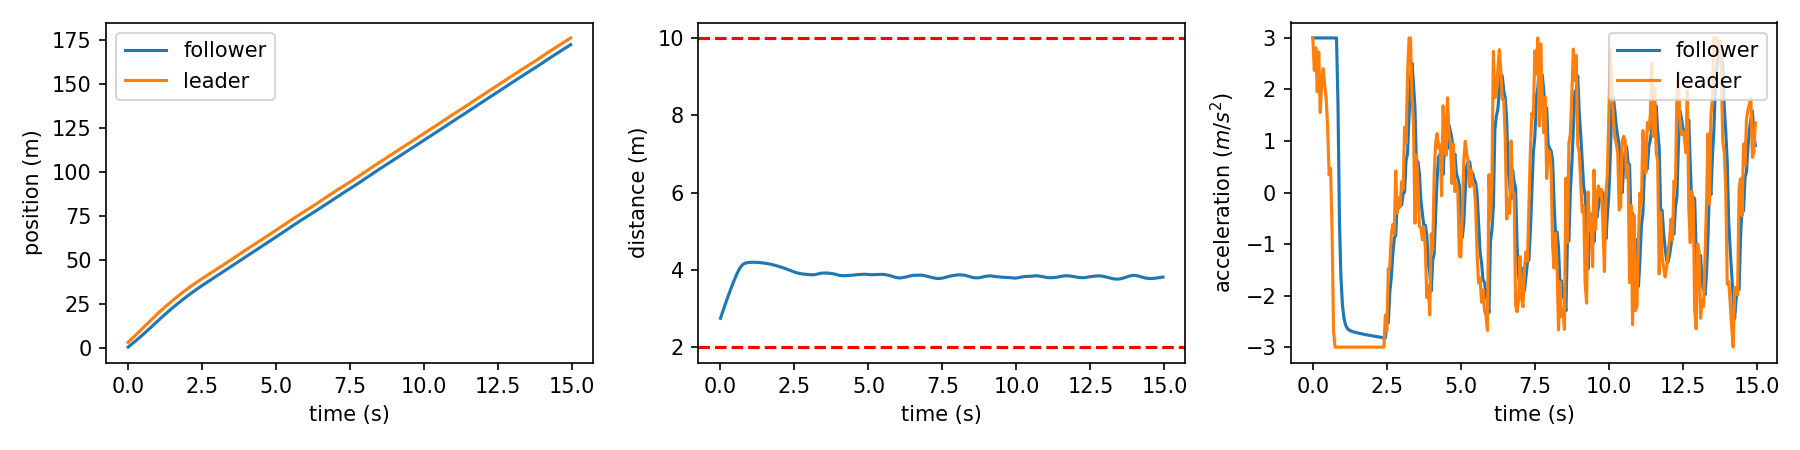
\includegraphics[width=13.8cm, keepaspectratio]{img/5_3_triplot_attacker.png}
	\caption{Initial configuration: $x_{l0}=2.63 \; m$, $v_{l0}=15.58 \frac{m}{s}$, $v_{f0}=13.28 \frac{m}{s}$. We can see how the attacker found the strategy of rapidly accelerating and breaking. The defender, though, succeeds in keeping its distance safe and almost constant over time.}
    \label{fig:single_triplot_attacker}
\end{figure}

\begin{figure}[H]
	\centering
	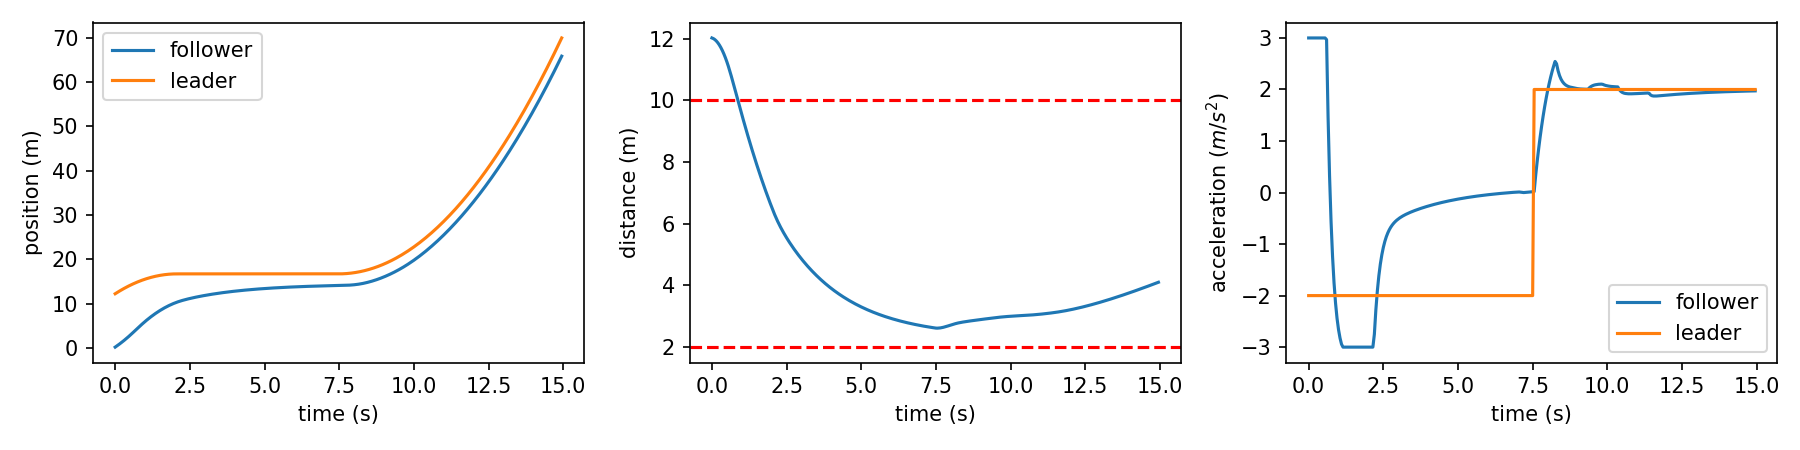
\includegraphics[width=13.8cm, keepaspectratio]{img/5_3_triplot_step_up.png}
	\caption{Initial configuration: $x_{l0}=12.03 \; m$, $v_{l0}=4.49 \frac{m}{s}$, $v_{f0}=4.41 \frac{m}{s}$. In this scenario the defender has the initial disadvantage of being too far from the leader. It safely closes the gap and is able to tolerate the sudden acceleration of the leader.}
    \label{fig:single_triplot_stepup}
\end{figure}

\begin{figure}[H]
	\centering
	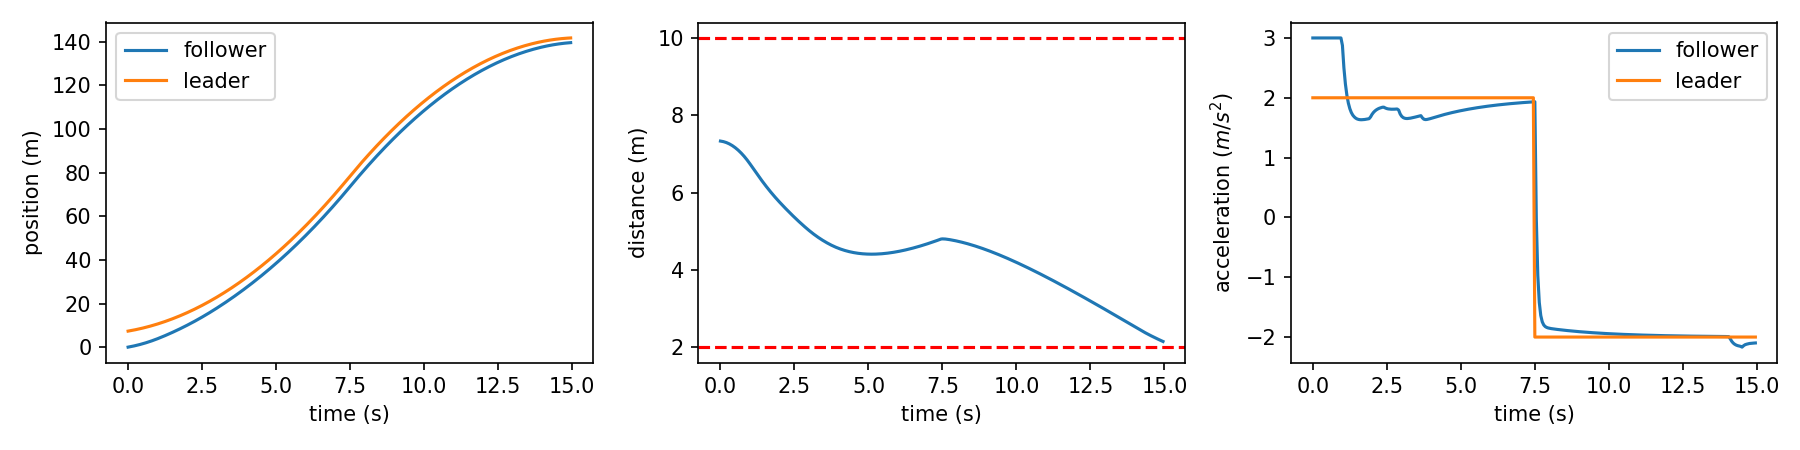
\includegraphics[width=13.8cm, keepaspectratio]{img/5_3_triplot_step_down.png}
	\caption{Initial configuration: $x_{l0}=7.33 \; m$, $v_{l0}=2.19 \frac{m}{s}$, $v_{f0}=2.21 \frac{m}{s}$. In this scenario the defender is able to tolerate quite well the sudden brake since it was keeping the evaluated safety distance.}
    \label{fig:single_triplot_stepdown}
\end{figure}

\begin{figure}[H]
	\centering
	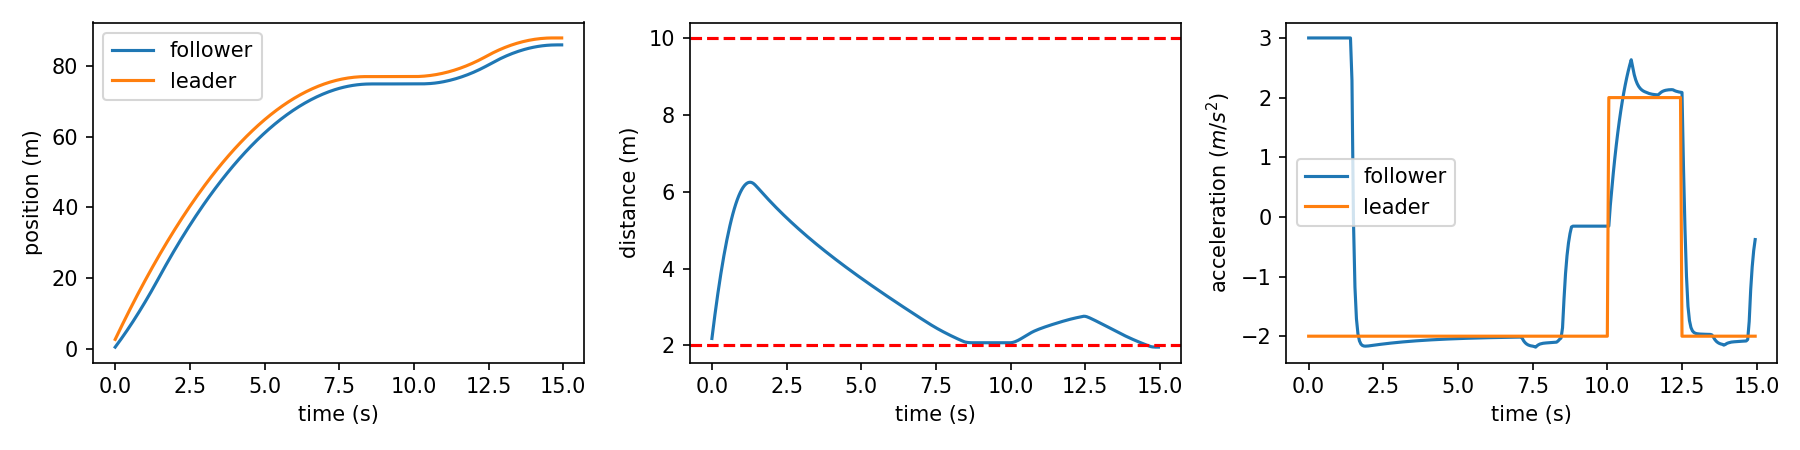
\includegraphics[width=13.8cm, keepaspectratio]{img/5_3_triplot_pulse.png}
	\caption{Initial configuration: $x_{l0}=2.63 \; m$, $v_{l0}=15.58 \frac{m}{s}$, $v_{f0}=13.28 \frac{m}{s}$. In this scenario of sudden acceleration and brake, the defender slowly approaches the opponent until it stops waiting for it to move. It adapts to the opponent behaviour arriving at the minimum allowed distance without violating the constraint.}
    \label{fig:single_triplot_pulse}
\end{figure}

It is possible to notice how well the follower manages the presented corner cases.
In the figure \ref{fig:single_triplot_attacker} we can see how the follower safely keeps an almost steady distance with a leader that behaves in a unpredictable way.
The follower mimics perfectly the acceleration pattern of the leader.
The same happens in the figure \ref{fig:single_triplot_stepdown} where, as soon as the leader suddenly brakes, the follower does the same to keep the safety distance.

In the figure \ref{fig:single_triplot_stepup}, it is interesting to notice how the follower is able to exploit the moments in which the leader is almost static in order to close the initial gap.
Even if the initial condition was not safe, the follower is able to recover from it and maintain the distance between the safety boundaries.

The follower, during the training, has learnt also to halt completely if the leader does so.
Such behaviour is visible in the figure \ref{fig:single_triplot_pulse} in which the follower halts in correspondence with the minimum distance allowed.

Even though the initial configuration plays a crucial role in the controller's safety, it is possible to observe how the NNs develop consistent strategies to solve at best their task.

In order to compare different models and have an estimate of their performances, we ran $10k$ simulation of different trajectories and, for each instant, we computed the percentage of them that was lying inside the given boundaries.
By using this kind of metrics it is possible to have a precise estimate of how well a given model is performing.

\begin{figure}[H]
	\centering
	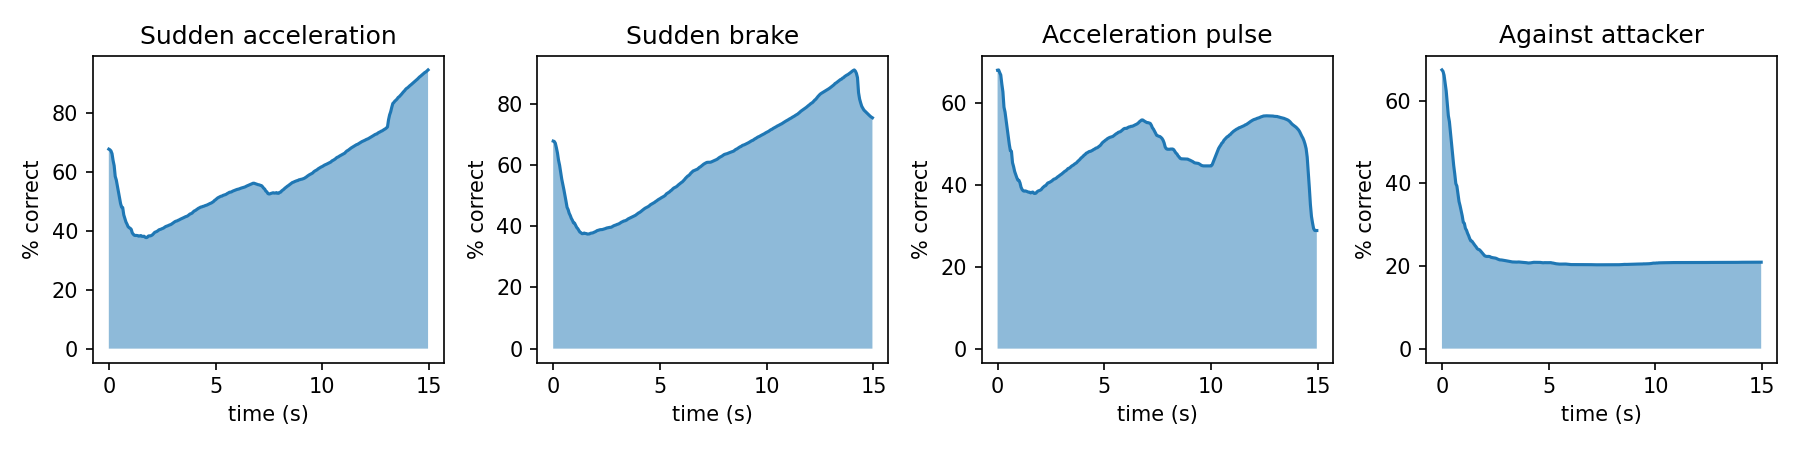
\includegraphics[width=13.8cm, keepaspectratio]{img/5_3_pct_histogram.png}
	\caption{Percentage of correct trajectories for each timestep. We can see that the trained model successfully control over the 80\% of the scenarios of sudden acceleration or brake. It behaves less well with the acceleration pulse and struggle against the attacker's behaviour. It is evident from the plot that in almost 40\% of the cases, the simulation start from forbidden conditions and this should be taken into account to evaluate the model.}
    \label{fig:pct_hist_single}
\end{figure}

It is worth mentioning that the figure \ref{fig:pct_hist_single} shows the results of simulations whose initial conditions have been sampled from the training intervals.
That is to say that, as we can read from the figure, the 30\% of the simulations starts from \textbf{unsafe} initial conditions.

\begin{figure}[H]
	\centering
	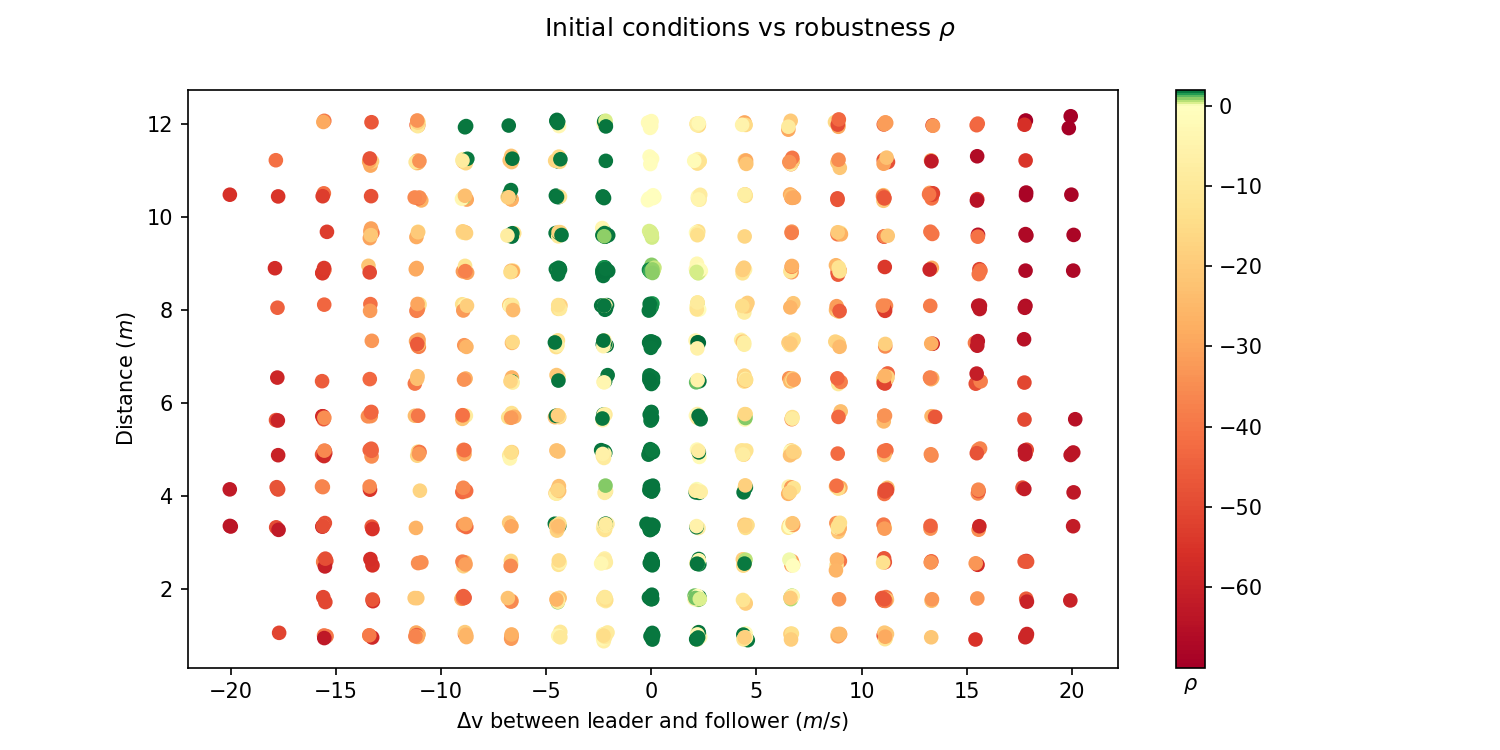
\includegraphics[width=14cm, keepaspectratio]{img/5_3_atk_scatterplot.png}
	\caption{Visualization of the simulations' robustness with respect to the sampled initial conditions. The scenario of the simulations is the one in which the leader is controlled by the attacker NN. This figure shows  the correlation between the initial conditions and the robustness of the defender NN. It is possible to notice how the defender manages very well the cases in which the two cars have similar initial velocity, given that the initial distance is inside the safety range. The  defender can catch up with the attacker even if the latter is further but only if the leader is not going too fast with respect to the follower.}
    \label{fig:atk_scatterplot}
\end{figure}

In the figure \ref{fig:atk_scatterplot} it is possible to notice how the \textit{attacker} is able to exploit favorable scenarios to push the \textit{defender} outside of the safety boundaries.
For instance, if the initial distance is already outside the boundaries and the \textit{attacker} is moving at a considerably different velocity with respect to the follower, it is not possible for the \textit{defender} to get to a safe state (as shown in the figure \ref{fig:atk_scatterplot}).
The \textit{attacker}'s ability to exploit favorable initial conditions could explain the poorer performances of the \textit{defender} in the simulations in which the leader car is controlled by the \textit{attacker} itself.

\subsubsection{One leader and $n$ followers}
Given a solution of the problem for two cars, it was straightforward to extend the application to the platooning of $n$ cars.
The idea is that each car in the line should follow the car in front.
At this stage it does not matter anymore if the car in front is an \textit{attacker} or a \textit{defender}: the aim of each follower is simply to follow.
In such a way it is possible to add an arbitrary number of followers to the line.

The two NNs trained with one leader and only one follower, whose result has been shown above, can be used separately to accomplish such task.
In particular, the only leader of the line will be controlled by the \textit{attacker} NN (or any other arbitrary controller), while all the followers will be controller by a copy of the same \textit{defender} NN.

\begin{figure}[H]
	\centering
	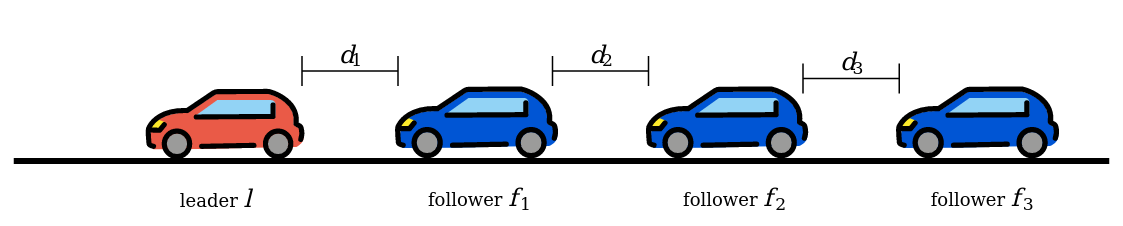
\includegraphics[width=12cm, keepaspectratio]{img/5_3_complete_platooning.png}
	\caption{The complete platooning setting, each car has knowledge of its status and the distance from the car in front.}
\end{figure}

In the tested setting there is only a leader $l$ followed by $3$ followers $f_1$, $f_2$ and $f_3$.
Each follower has to keep the respective distance $d_1$, $d_2$ and $d_3$ with the vehicle in front within the safety range.
In such setting, the leader can be controlled by the \textit{attacker} NN or any adversarial policy.
The follower, instead, are controlled separately by the \textit{defender} NN.

The vehicles start equispaced with an initial distance $d_{init}= d_1 = d_2 = d_3$ drawn from a $\mathcal{U}(1,8)$ distribution.
Similarly, the initial velocity $v_{init}$ of the cars is drawn from a $\mathcal{U}(1,5)$ distribution and is the same for all of them.

We performed the simulations for the whole platoon in the same settings used for the basic case.
The results are shown in the figures from \ref{fig:multi_triplot_attacker} to \ref{fig:multi_triplot_pulse}.
\begin{figure}[H]
	\centering
	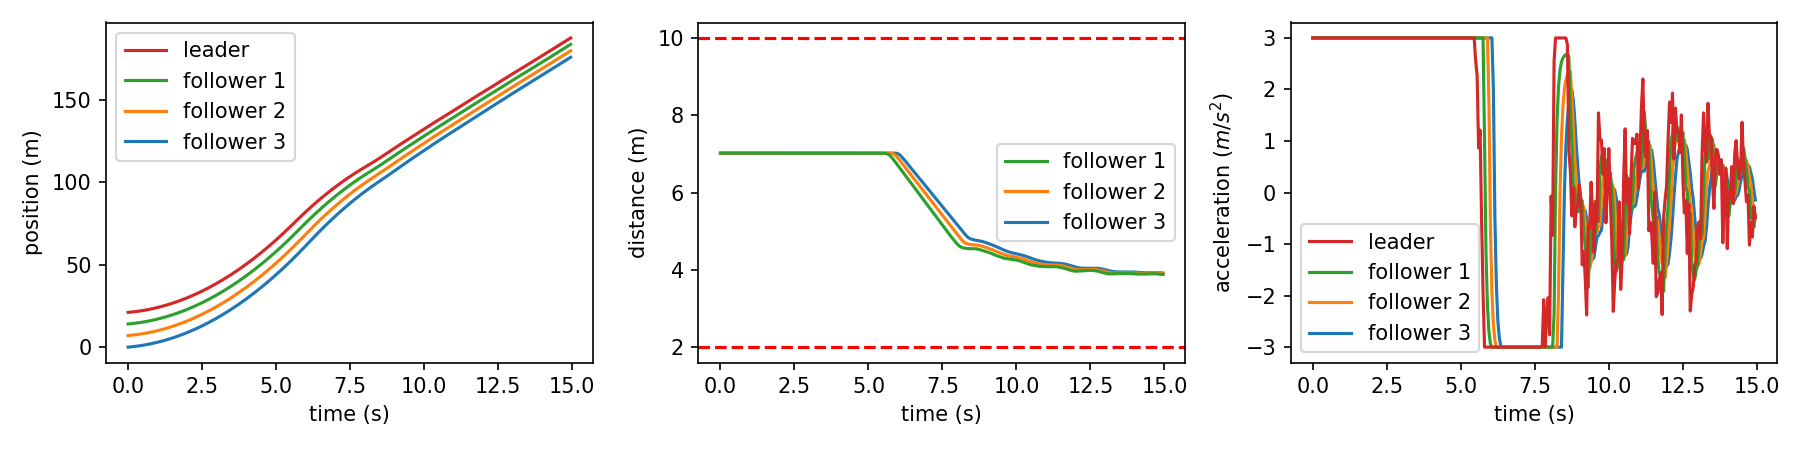
\includegraphics[width=13.8cm, keepaspectratio]{img/5_3_triplot_fullplatooning_attacker.png}
	\caption{Initial configuration: $d_{init}= 7.01\; m$, $v_{init}=1.30 \frac{m}{s}$. We can see how the attacker tries two strategies (sudden brake and rapid acceleration/brake sequence), but the platoon can still manage the situation safely.}
    \label{fig:multi_triplot_attacker}
\end{figure}

\begin{figure}[H]
	\centering
	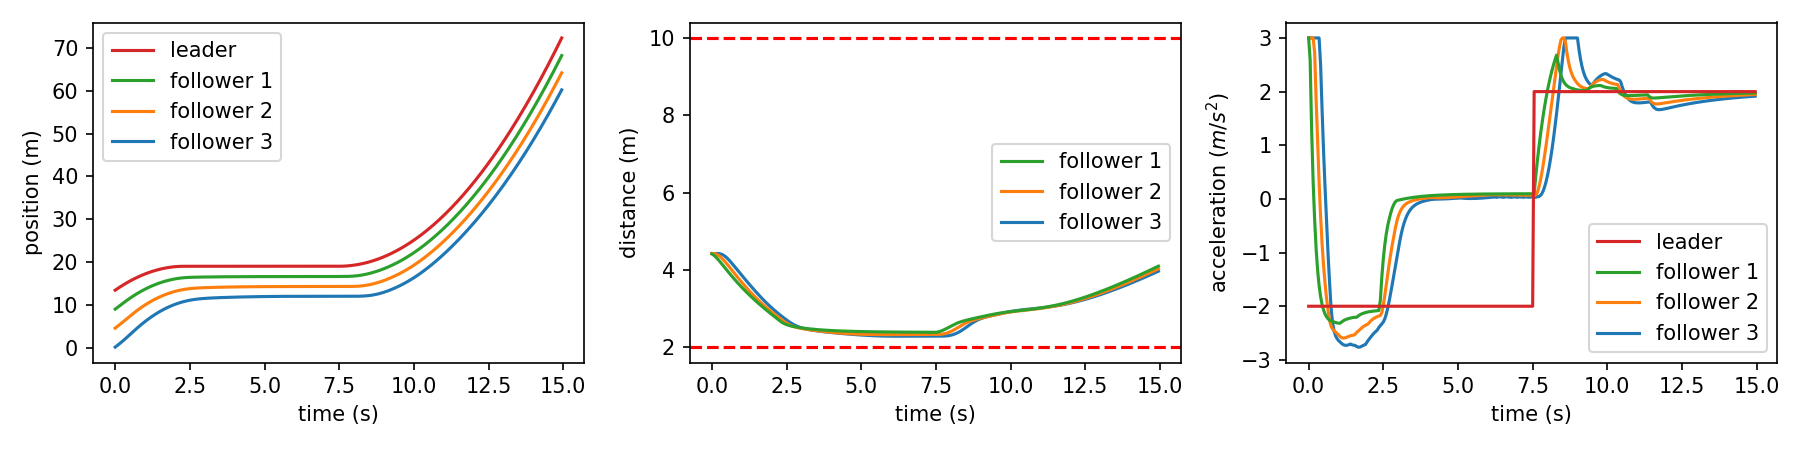
\includegraphics[width=13.8cm, keepaspectratio]{img/5_3_triplot_fullplatooning_stepup.png}
	\caption{Initial configuration: $d_{init}= 4.42\; m$, $v_{init}=4.99 \frac{m}{s}$. It is worth noticing how the whole platoon stops at some point still keeping a safe distance. It restarts right after and hold the safety distance for the rest of the simulation.}
    \label{fig:multi_triplot_stepup}
\end{figure}

\begin{figure}[H]
	\centering
	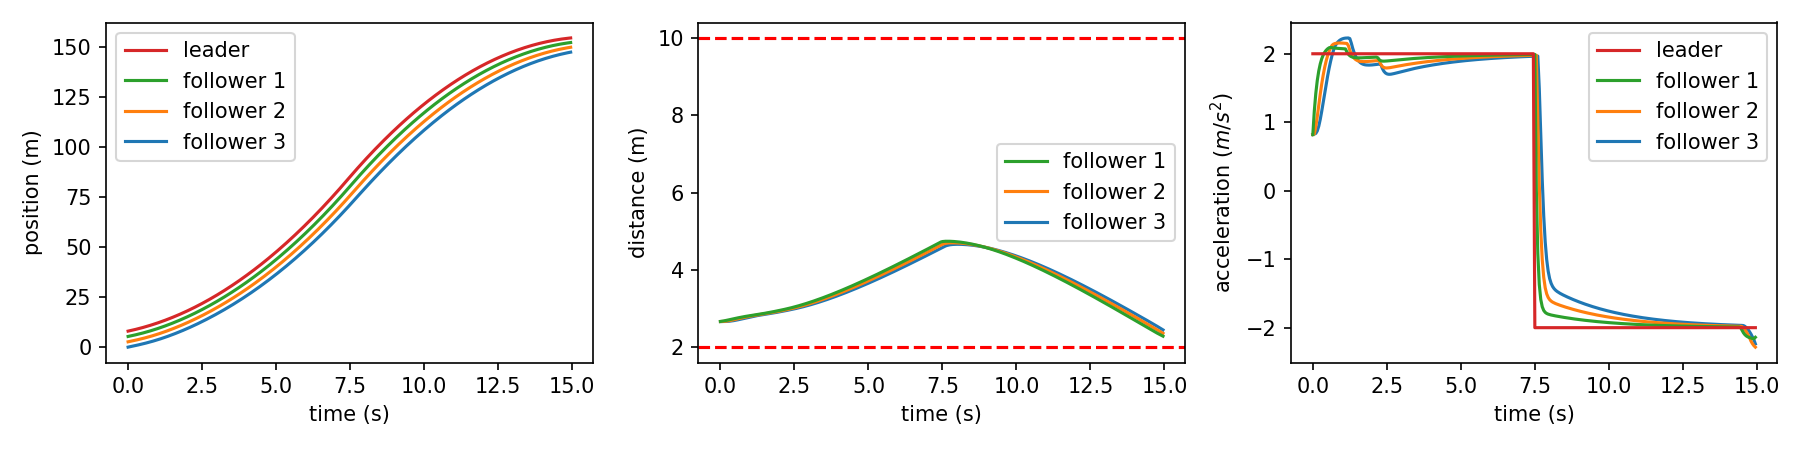
\includegraphics[width=13.8cm, keepaspectratio]{img/5_3_triplot_fullplatooning_stepdown.png}
	\caption{Initial configuration: $d_{init}= 2.66\; m$, $v_{init}=3.01 \frac{m}{s}$. The trajectories are robust despite the sudden brake of the leader.}
    \label{fig:multi_triplot_stepdown}
\end{figure}

\begin{figure}[H]
	\centering
	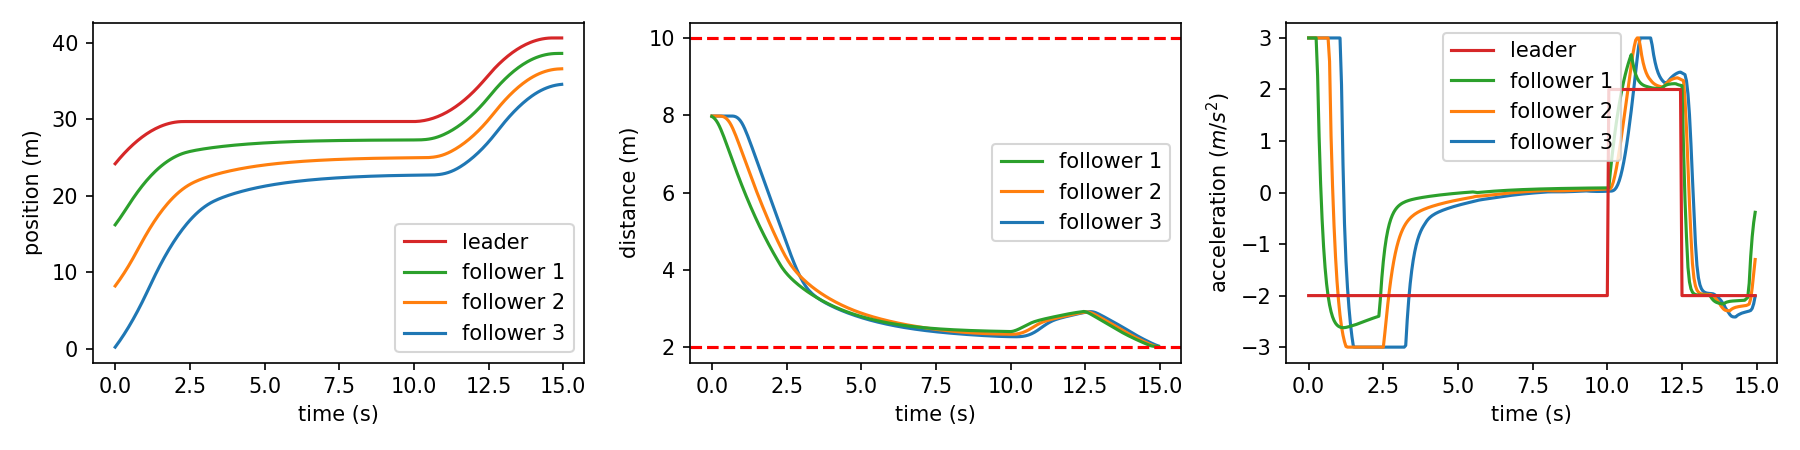
\includegraphics[width=13.8cm, keepaspectratio]{img/5_3_triplot_fullplatooning_pulse.png}
	\caption{Initial configuration: $d_{init}= 7.97\; m$, $v_{init}=4.96 \frac{m}{s}$. The whole platoon reacts interestingly to the sudden changes. As it would happen in the real world, getting further from the head of the platoon, the accelerations changes appear damped and here it is clearly visible.}
    \label{fig:multi_triplot_pulse}
\end{figure}
The platoon's followers behave exactly like the follower of the simple case with one leader and one follower.
This is not surprising since they all use the same NN as controller.

	\chapter{Conclusions and future works}

\section{Summary}
The potential of the newest models of machine learning in the CPS field is underexploited: while in controlled scenarios many classical control methods are still effective, in open world scenarios they are not always a viable option.
Better alternatives like reinforcement learning, though promising, struggle to give an adequate safety guarantee for real-world applications.

We wanted to address such problem drawing inspiration from GANs literature: two opposing NNs that learn from each other.
The outcome of the learning procedure is one \textbf{defender} NN that is able to face in a safe and robust way the scenarios generated by the \textbf{attacker} NN.

We tested our method in two different settings: the traditional \textbf{cruise control} problem and  the \textbf{platooning} one.


\section{Conclusions}
In both the case studies, our architecture behaved well and showed promising results, a potential for further research on the topic.

With the presented architecture we showed a possible way of achieving both safety and interpretability of the model.
The \textit{defender}, in fact, can safely overcome most of the presented situations, some of which are indeed unrealistic corner-cases.
The \textit{attacker}, on the other side, is able to give insight on which are the most insidious configurations of the environment, allowing to deploy better systems to face them.

The architecture proved itself to be robust even in case of sparse exploration of the space of the initial configuration.
Starting for an unknown state, in fact, is almost always able to reach a known and safe state.

The results presented are encouraging.

\section{Future work}
The presented architecture is quite complex and requires a deeper exploration in order to uncover the full potential.

The architecture would greatly benefits of some optimizations to enable the processing of simulations \textit{mini-batches} in parallel.

It would be interesting to try the architecture on different CPS and different problems.
A possible future development, in fact, could be to apply this architecture to control non-differentiable models.
It could be achieved by training a differentiable NN as a surrogate of the non-differentiable system and use it as model $\mathcal{M}$.

Another matter that requires more attention is the choice of the points on the \textit{hyper-grid} for the training.
While at the moment we sample it uniformly, other smarter strategies could be applied since not every configuration is equally probable.

    \renewcommand{\bibsection}{\chapter*{References}}
    \markboth{\MakeUppercase{References}}{}
    \addcontentsline{toc}{chapter}{References}
    \bibliographystyle{unsrt}
    \bibliography{refs}

\end{document}
